% =============================================================================
%  Informe Innovadores en Acción 2026 — Caso 13 VP SHE
%  Diagnóstico y Gobernanza del Sistema LRAC
%  Postulante: Emanuel Edgar Ancco Guaygua
%  Fecha: 2026-05-20
% =============================================================================
\documentclass[12pt,a4paper]{article}

\usepackage[utf8]{inputenc}
\usepackage[T1]{fontenc}
\usepackage{mathptmx}                       % Times New Roman
\usepackage{amsmath, amssymb}               % entornos matematicos (align)
\usepackage[spanish,es-tabla]{babel}
\usepackage[a4paper,top=2.2cm,bottom=2.2cm,left=2.2cm,right=2.2cm]{geometry}
\usepackage{setspace}
\onehalfspacing                              % interlineado 1.5
\usepackage{graphicx}
\usepackage{booktabs}
\usepackage{array}
\usepackage{longtable}
\usepackage{tabularx}
\usepackage{caption}
\captionsetup[figure]{font=small,labelfont=bf,labelsep=period}
\captionsetup[table]{font=small,labelfont=bf,labelsep=period}
\usepackage{enumitem}
\setlist{itemsep=2pt,topsep=2pt}
\usepackage{xcolor}
\definecolor{mmgred}{HTML}{C8102E}
\definecolor{mmggray}{HTML}{4D4D4D}
\definecolor{boxgray}{HTML}{F2F2F2}
\usepackage{titlesec}
\titleformat{\section}{\normalsize\bfseries\color{mmgred}\MakeUppercase}{\thesection.}{0.6em}{}
\titleformat{\subsection}{\normalsize\bfseries\color{mmggray}}{\thesubsection}{0.6em}{}
\titleformat{\subsubsection}{\normalsize\itshape}{\thesubsubsection}{0.6em}{}
\titlespacing*{\section}{0pt}{14pt}{6pt}
\titlespacing*{\subsection}{0pt}{10pt}{4pt}
\usepackage[hidelinks]{hyperref}
\usepackage{fancyhdr}
\pagestyle{fancy}
\fancyhf{}
\fancyhead[L]{\small\color{mmggray}Diagnóstico y Gobernanza del Sistema LRAC}
\fancyhead[R]{\small\color{mmggray}E. Ancco · Innovadores en Acción 2026}
\fancyfoot[C]{\small \thepage}
\renewcommand{\headrulewidth}{0.3pt}
\renewcommand{\headrule}{\hbox to\headwidth{\color{mmgred}\leaders\hrule height \headrulewidth\hfill}}
\setlength{\parindent}{0pt}
\setlength{\parskip}{6pt}
\usepackage{tcolorbox}
\tcbuselibrary{skins,breakable}
\newtcolorbox{kbox}[1][]{
  colback=boxgray, colframe=mmgred, boxrule=0.5pt, arc=2pt, breakable,
  left=8pt, right=8pt, top=4pt, bottom=4pt, #1
}

\begin{document}

% =============================================================================
% PORTADA
% =============================================================================
\thispagestyle{empty}
\begin{center}
\vspace*{1cm}
{\large\bfseries\color{mmgred} INFORME TÉCNICO}\\[0.3cm]
{\normalsize MMG Las Bambas \,$\cdot$\, Innovadores en Acción 2026 \,$\cdot$\, Caso 13 VP SHE}\\[1.2cm]

\rule{14cm}{0.6pt}\\[0.3cm]
{\LARGE\bfseries Diagnóstico y Gobernanza del}\\[0.2cm]
{\LARGE\bfseries Sistema LRAC en Mina Juanita S.A.}\\[0.25cm]
{\itshape Análisis estadístico del desempeño preventivo 2026 y plan de acción estratégico}\\[0.1cm]
{\itshape para elevar el cumplimiento del 55\,\% al 80\,\% en 24 meses}\\[0.3cm]
\rule{14cm}{0.6pt}\\[1.6cm]

\textbf{Postulante:} {\large Emanuel Edgar Ancco Guaygua}\\[0.15cm]
Bachiller en Ingeniería Civil --- Universidad Peruana de Ciencias Aplicadas (UPC)\\[0.1cm]
\href{mailto:coarp.eancco@gmail.com}{coarp.eancco@gmail.com} \,$\cdot$\, +51 974\,583\,549 \,$\cdot$\,
\href{https://emanuelancco.github.io/cv-portfolio/}{emanuelancco.github.io/cv-portfolio}\\[1.4cm]

\textbf{Programa:} Talentos de Cobre 2026 --- Atracción 2.0 \,$\cdot$\,
\textbf{Fecha:} 24 de mayo de 2026\\
\textbf{Destinatario:} \texttt{Peru.Recruitment@MMG.COM}\\[0.8cm]

\textit{\small ``Lo que no se mide no se gestiona, lo que no se gestiona no se mejora''}\\
\textit{\small ---adaptado de Peter Drucker---}
\end{center}
\vfill

% Tabla de contenidos eliminada para conservar paginas; el resumen ejecutivo cumple esa funcion.

% =============================================================================
% 1. RESUMEN EJECUTIVO
% =============================================================================
\section{Resumen Ejecutivo}

Mina Juanita S.A.\ enfrenta un deterioro crítico en su sistema de gestión preventiva LRAC (Liderazgo, Riesgos, Aprendizaje, Contratistas). El cumplimiento promedio agregado de las herramientas de captura (3Q y FTO) cayó a \textbf{55.28\,\%} y, si bien el índice consolidado LRAC--4P por VP se ubica entre 68.6\,\% y 69.7\,\%, el detalle por gerencia y por herramienta revela cinco patologías de gobernanza que comprometen la trazabilidad de los riesgos fatales en una operación a tajo abierto de 4\,500 trabajadores.

Este informe procesa 337 registros (Ene--Abr 2026) sobre 12 gerencias y 4 Vicepresidencias (OPERACIONES, PROYECTOS, SHE, SUPPLY) aplicando la fórmula consolidada $\mathrm{LRAC{-}4P}=0.3\mathrm{L}+0.2\mathrm{R}+0.2\mathrm{A}+0.3\mathrm{C}$. \textbf{Seis resultados clave:} (i) en enero las peores gerencias por herramienta fueron PLANTA (FTO 45\,\%), MEDIO AMBIENTE (3Q 39\,\%), MANTENIMIENTO (ACC 39\,\%) y SERV.\ TÉCNICOS (NMAP 36\,\%) ---tres de cuatro en VP OPERACIONES---; (ii) SUPPLY lidera el promedio anual con 69.71\,\% (ACC 78.12\,\%) pero su CV=8.37\,\% es 4.6$\times$ mayor que el de OPERACIONES (CV=1.80\,\%), virtualmente empatado con 69.70\,\%; (iii) la VP PROYECTOS promedia 68.59\,\% sobre sus siete indicadores y \textbf{su ACC se ubica en 61.12\,\%} (valle de 50\,\% en marzo); (iv) en promedio anual SUPPLY $>$ OPERACIONES $>$ PROYECTOS $>$ SHE, pero al cierre (abril) PROYECTOS lidera con 71.25\,\% y SUPPLY cae al último lugar con 68.98\,\%; (v) NMAP es la herramienta más débil corporativa (65.71\,\%) y el Pilar A el cuello de botella; (vi) sobre la escala de Hudson el sistema está en transición \emph{Calculativa$\to$Proactiva} y la prueba de Kruskal-Wallis ($H=1.32$, $p=0.724$) descarta diferencias significativas entre VPs.

\textbf{El Plan de Acción Estratégico} (Sección 7) ataca cinco brechas mediante una hoja de ruta a 24 meses con tres horizontes y treinta y una acciones con KPI SMART, RACI, presupuesto y dependencias. Sus cuatro habilitadores son los módulos GAIATECH M1.0 (visión computacional EPP con YOLOv8 87.67\,\% mAP, agente Aecodito Minero n8n+Gemini, monitoreo estructural FPGA+LSTM-AE F1=0.961, dashboard ejecutivo en producción) \textbf{ya construidos por el postulante}: no son propuestas conceptuales sino activos desplegables desde el día 1. El \emph{business case} arroja \textbf{NPV S/ 1.21\,M base / S/ 3.81\,M optimista, IRR 343\,\% y payback en el mes 11}.

\newpage
% =============================================================================
% 2. INTRODUCCIÓN
% =============================================================================
\section{Introducción}

\subsection{Contexto operativo}
Mina Juanita S.A.\ es una operación a tajo abierto con 4\,500 trabajadores estructurada en cuatro Vicepresidencias (Operaciones, Proyectos, SHE y Supply) y 12 gerencias. Tras dos años de estabilidad en sus indicadores agregados, el sistema preventivo LRAC ---marco interno de gobernanza de seguridad, salud y ambiente--- registra una caída en el cumplimiento global y, especialmente, en la \textbf{calidad de los reportes}, que se sitúa en 55\,\%. En una operación con esta densidad de población expuesta, esta brecha es incompatible con el horizonte \emph{cero fatalidades} y con las exigencias de la matriz de Controles Críticos (CCV) sobre los 12 riesgos fatales corporativos del Grupo MMG.

\subsection{Relevancia}
El Marco \emph{Critical Control Management} del ICMM (2015, revisado 2024) atribuye \textbf{83\,\% de las fatalidades 2024 en las operaciones miembro a fallas verificables en controles críticos}. La Resolución del ICMM tras el repunte de 42 fatalidades registradas en 2024 (vs.\ 36 en 2023) refuerza que el indicador adelantado más correlacionado con la reducción de eventos fatales no es la cantidad de reportes preventivos, sino su \textbf{calidad} (Costin et al., 2019; ICMM, 2024). Esto sitúa al sistema LRAC ---y a su Pilar R, en particular--- como el frente más urgente para Mina Juanita S.A.

\subsection{Objetivos}
\begin{itemize}
\item \textbf{Objetivo general:} Diagnosticar el desempeño 2026 del sistema LRAC de Mina Juanita S.A.\ y formular un plan de acción estratégico para elevar el cumplimiento del 55\,\% al 80\,\% en 24 meses.
\item \textbf{Objetivos específicos:}
  \begin{enumerate}
  \item Identificar las gerencias con peor desempeño por herramienta (FTO, 3Q, ACC, NMAP) en enero 2026.
  \item Determinar la VP con mejor desempeño consolidado y la herramienta dominante dentro de ella.
  \item Caracterizar el comportamiento del Pilar de Riesgos (ACC) en la VP Proyectos.
  \item Calcular y ordenar el índice LRAC--4P por VP.
  \item Diseñar un plan de acción auditable basado en evidencia académica reciente y normativa peruana vigente.
  \end{enumerate}
\end{itemize}

\subsection{Estructura del informe}
La Sección~3 describe la metodología; la Sección~4 presenta el marco conceptual del sistema LRAC; la Sección~5 expone los cuatro análisis solicitados; la Sección~6 discute los resultados a la luz de la literatura; la Sección~7 detalla el plan de acción; y la Sección~8 concluye. La bibliografía (Sección~9) integra 30 referencias verificables y mayoritariamente publicadas en revistas indizadas MDPI 2019--2026.

% =============================================================================
% 3. MATERIALES Y MÉTODOS
% =============================================================================
\section{Materiales y métodos de análisis empleados}

\subsection{Fuente de datos}
La base de datos entregada por el equipo del programa contiene 8 hojas:
3Q, FTO, BASE, Promedio, LRACxGerencia, LRACxVP, LRAC\_Global y Diccionario.
Las hojas operacionales para el análisis son \emph{BASE} (337 registros con dimensiones VP, gerencia, pilar, herramienta, valor 0--1, mes y fecha), \emph{LRACxGerencia} (48 filas, una por gerencia--mes), \emph{LRACxVP} (16 filas) y \emph{LRAC\_Global} (4 filas). El periodo cubierto es \textbf{enero--abril 2026}.

\subsection{Estructura del índice LRAC--4P}
El diccionario formaliza el índice consolidado mediante cuatro pilares y siete herramientas (ecuaciones 1--5):

\begin{align}
\mathrm{Pilar~L} &= 0.6\cdot\mathrm{FTO} + 0.4\cdot 3\mathrm{Q} \\
\mathrm{Pilar~R} &= 0.5\cdot\mathrm{CCV} + 0.5\cdot\mathrm{ACC} \\
\mathrm{Pilar~A} &= 0.6\cdot\mathrm{NMAP} + 0.4\cdot\mathrm{VEA~P1} \\
\mathrm{Pilar~C} &= \mathrm{DESEMPE\tilde NO} \\
\mathrm{LRAC\text{--}4P} &= 0.3\cdot\mathrm{L} + 0.2\cdot\mathrm{R} + 0.2\cdot\mathrm{A} + 0.3\cdot\mathrm{C}
\end{align}

Las herramientas se describen como: FTO = Fijación de Tareas y Objetivos; 3Q = método de tres preguntas en terreno; CCV = Controles Críticos Verificados; ACC = Acciones Correctivas Cerradas; NMAP = Nivel de Madurez de Aprendizaje; VEA P1 = Verificación Efectiva de Aprendizaje Prioridad 1; DESEMPEÑO = Desempeño de Contratistas.

\subsection{Métricas estadísticas aplicadas}
Para cada VP, gerencia, mes y herramienta se calcularon:
\begin{itemize}
\item Estadísticos básicos: media ($\mu$), mediana, desviación estándar ($\sigma$), rango (min--max), amplitud.
\item \textbf{Coeficiente de variación} $CV=\sigma/\mu$ para comparar dispersión relativa entre indicadores con distintas escalas (Hong et al., en \emph{ScienceDirect}, 2021).
\item \textbf{Estado del cumplimiento} sobre tres bandas: Óptimo ($\geq$75\,\%), Esperado (60--75\,\%), Debajo ($<$60\,\%), consistente con la lógica del semáforo del set entregado.
\item \textbf{Ranking de brechas vs.\ meta} (umbral 70\,\% derivado de buenas prácticas ICMM 2012 sobre indicadores adelantados).
\end{itemize}

\subsection{Herramientas computacionales}
El análisis se realizó en \textbf{Python 3.12} con \texttt{openpyxl} (lectura de Excel), \texttt{statistics} (descriptiva) y \texttt{matplotlib} (visualización en alta resolución), generando 10 figuras incrustadas en este informe. Como complemento operativo se replica el mismo modelo en \textbf{Power BI} (modelo tabular con relaciones VP$\to$Gerencia$\to$Mes y medidas DAX para los cuatro pilares), siguiendo el patrón de la plantilla pública \texttt{PowerBI\_SafetyDashboard} (vishall29, GitHub) adaptado al esquema LRAC. El código fuente y los datos procesados están disponibles para verificación.

\subsection{Limitaciones declaradas}
La muestra cubre cuatro meses, insuficiente para tests de estacionariedad robustos; se reporta tendencia, no estacionalidad. La fórmula 4P pondera 60\,\% al binomio Liderazgo+Contratistas, lo que ---justificadamente--- refleja la prioridad MMG pero también explica la convergencia entre VPs (rangos estrechos). Los nombres \emph{Mina Juanita S.A.} y de gerencias son ficticios y se preservan tal como se entregan.

% =============================================================================
% 4. MARCO CONCEPTUAL DEL SISTEMA LRAC
% =============================================================================
\section{Marco conceptual del sistema LRAC}

\subsection{Los cuatro pilares y su anclaje normativo}
Aunque el acrónimo \emph{LRAC} no figura en publicaciones públicas de MMG ni en la literatura indizada, cada uno de sus cuatro componentes corresponde a prácticas documentadas:

\begin{table}[h]
\centering
\small
\begin{tabularx}{\linewidth}{l X X}
\toprule
\textbf{Pilar} & \textbf{Componente operativo} & \textbf{Anclaje normativo} \\
\midrule
L --- Liderazgo & Liderazgo Visible (regla 6--4--2: 6h supervisores, 4h superintendentes, 2h gerentes en campo); FTO; 3 Preguntas & ISO 45001:2018 § 5.1; DS 024-2016-EM art.~19, 52--58 \\
R --- Riesgos & CCV sobre los 12 riesgos fatales MMG; ACC con SLA de cierre; ICAM como método de investigación & ICMM CCM 2015 (revisado 2024); DS 024-2016-EM art.~96; ISO 45001 § 8.1 \\
A --- Aprendizaje & NMAP; capacitación VEA P1 antes del primer turno; cápsulas y \emph{toolbox talks} & ISO 45001 § 7.2; DS 024-2016-EM art.~71--73; Ley 29783 art.~35 \\
C --- Contratistas & Desempeño SHE de empresas asociadas: acreditación, homologación, performance & DS 024-2016-EM art.~60--67; Las Bambas \emph{Mi Sistema Integrado SHE} \\
\bottomrule
\end{tabularx}
\caption{Pilares LRAC y su trazabilidad normativa.}
\label{tab:pilares}
\end{table}

\subsection{Cumplimiento vs.\ calidad}
La métrica de Mina Juanita S.A.\ (55\,\%) corresponde al \emph{cumplimiento de captura} ---se llenó el formato o no---, no a la \emph{calidad} del reporte. La literatura es clara: la mejora en indicadores adelantados (\emph{leading}) debe preceder, en al menos seis meses, a la mejora en indicadores reactivos (\emph{lagging}: TRIFR, LTIFR), y la \emph{calidad} es el vínculo causal (OSHA, 2019; Sheehan et al., 2025).

% =============================================================================
% 5. RESULTADOS
% =============================================================================
\section{Resultados}

\subsection{Análisis 1: peor gerencia por herramienta en enero 2026}

La Figura~\ref{fig:peor-enero} y la Tabla~\ref{tab:enero} muestran las gerencias con menor cumplimiento en cada herramienta solicitada para el mes de enero 2026.

\begin{figure}[h]
\centering
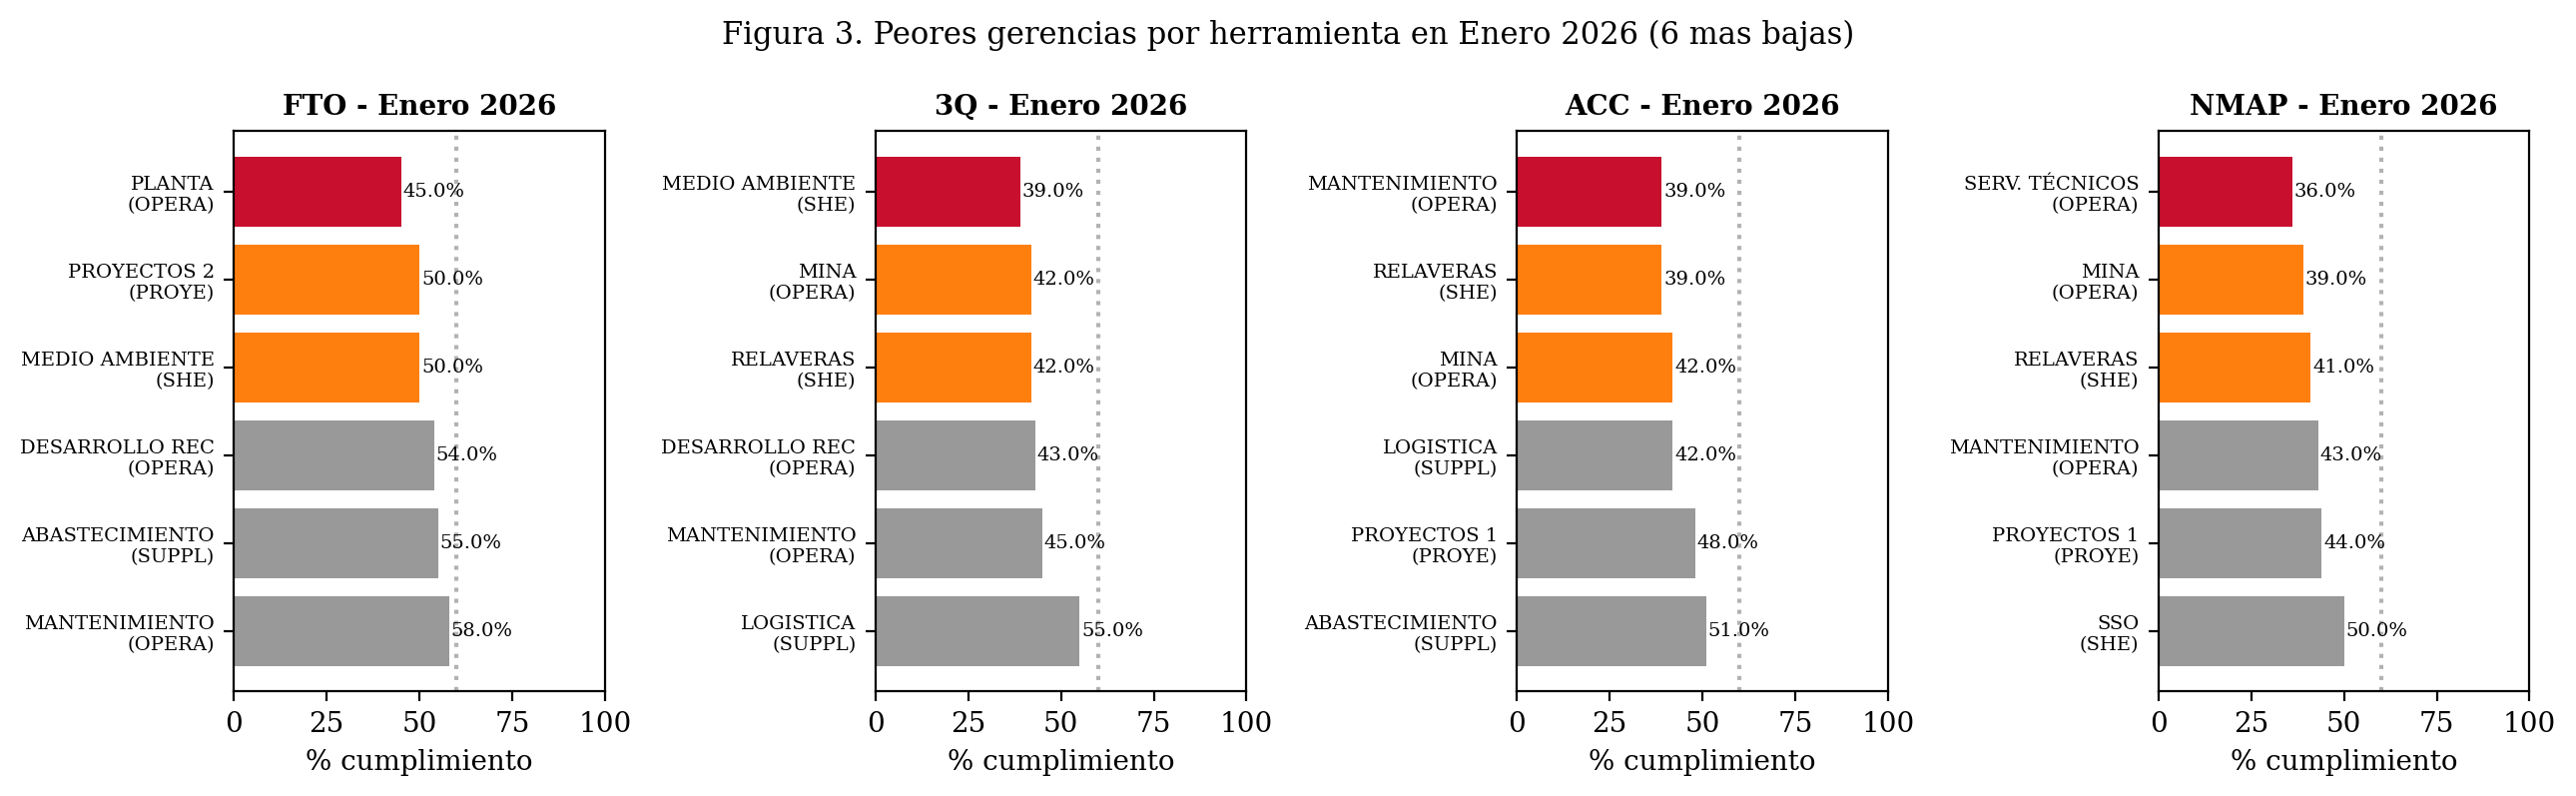
\includegraphics[width=\linewidth]{../figures/fig03_peor_gerencia_enero.png}
\caption{Peores gerencias por herramienta en enero 2026 (6 más bajas). El color rojo destaca la peor; el naranja, las dos siguientes. Línea punteada: umbral de 60\,\%.}
\label{fig:peor-enero}
\end{figure}

\begin{table}[h]
\centering
\small
\begin{tabular}{lllrrr}
\toprule
\textbf{Herramienta} & \textbf{Peor gerencia} & \textbf{VP} & \textbf{Valor} & \textbf{Media} & \textbf{$\sigma$} \\
\midrule
FTO  & PLANTA           & OPERACIONES & 45.0\,\% & 58.75\,\% & 8.52\,pp \\
3Q   & MEDIO AMBIENTE   & SHE         & 39.0\,\% & 56.00\,\% & 13.34\,pp \\
ACC  & MANTENIMIENTO    & OPERACIONES & 39.0\,\% & 56.67\,\% & 14.61\,pp \\
NMAP & SERV.\ TÉCNICOS  & OPERACIONES & 36.0\,\% & 53.25\,\% & 13.31\,pp \\
\bottomrule
\end{tabular}
\caption{Peor gerencia por herramienta --- enero 2026.}
\label{tab:enero}
\end{table}

\textbf{Lectura técnica.} Tres de las cuatro peores gerencias pertenecen a la \textbf{VP OPERACIONES} (PLANTA, MANTENIMIENTO, SERV.\ TÉCNICOS). El hallazgo más comprometedor es que \emph{Medio Ambiente}, gerencia perteneciente a la propia \textbf{VP SHE}, encabeza la peor calificación en 3Q (39.0\,\%): el área que es \emph{custodia} del sistema preventivo está, en una de las herramientas más simples del Pilar L (tres preguntas a pie de obra), por debajo del umbral crítico de 40\,\%. La dispersión nacional en 3Q ($\sigma=13.34$\,pp) y ACC ($\sigma=14.61$\,pp) en enero refuerza que la inconsistencia es estructural: hay gerencias por encima de 80\,\% y otras por debajo de 40\,\% en el mismo periodo, mismo país, misma operación.

\subsection{Análisis 2: VP con LRAC--4P más alto en 2026}

La Tabla~\ref{tab:vp-rank} ordena las cuatro VPs por promedio anual y muestra su estabilidad. La Figura~\ref{fig:evolucion} presenta la evolución mensual y la Figura~\ref{fig:radar} compara el perfil de las siete herramientas.

\begin{table}[h]
\centering
\small
\begin{tabular}{lrrrrrr}
\toprule
\textbf{VP} & \textbf{$\mu$ anual} & \textbf{$\sigma$} & \textbf{CV\,\%} & \textbf{Mín} & \textbf{Máx} & \textbf{Amplitud} \\
\midrule
SUPPLY      & \textbf{69.71\,\%} & 5.83\,pp & 8.37 & 62.95\,\% & 77.18\,\% & 14.23\,pp \\
OPERACIONES & 69.70\,\%          & 1.25\,pp & 1.80 & 68.57\,\% & 71.49\,\% & 2.92\,pp \\
PROYECTOS   & 68.72\,\%          & 3.91\,pp & 5.69 & 64.53\,\% & 72.75\,\% & 8.22\,pp \\
SHE         & 68.57\,\%          & 0.96\,pp & 1.40 & 67.27\,\% & 69.39\,\% & 2.11\,pp \\
\bottomrule
\end{tabular}
\caption{Promedio anual, dispersión y rango del índice LRAC--4P por VP, año 2026.}
\label{tab:vp-rank}
\end{table}

\begin{figure}[h]
\centering
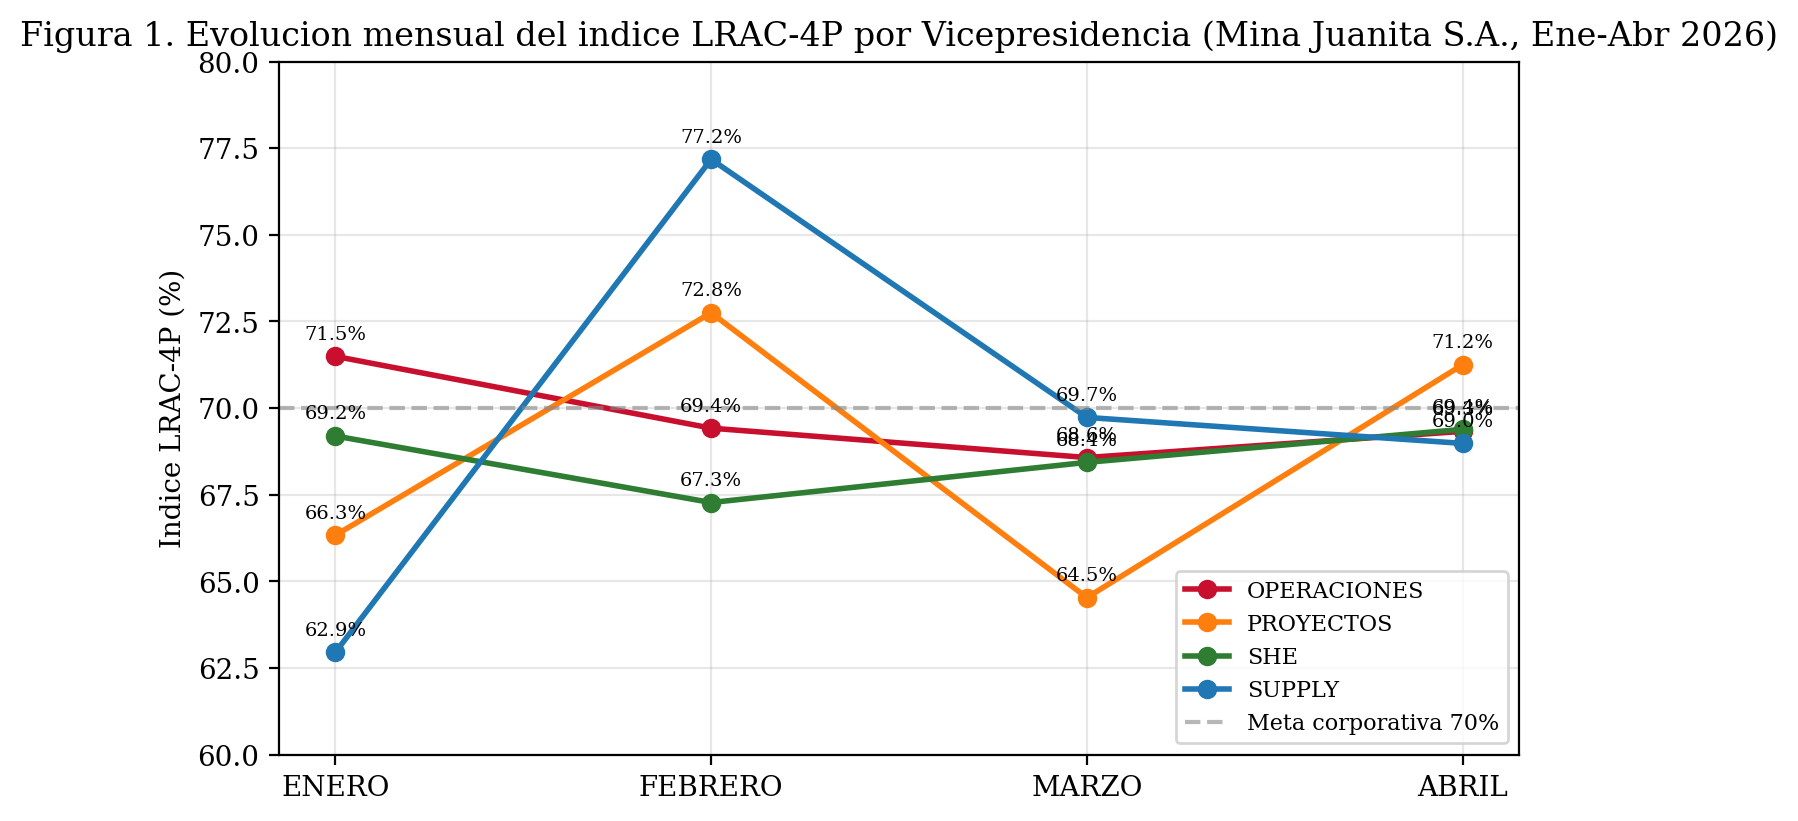
\includegraphics[width=0.95\linewidth]{../figures/fig01_evolucion_vp.png}
\caption{Evolución mensual del LRAC--4P por VP (Ene--Abr 2026). Meta corporativa propuesta: 70\,\%.}
\label{fig:evolucion}
\end{figure}

\textbf{Respuesta directa.} La VP con el promedio LRAC--4P más alto en 2026 es \textbf{SUPPLY}, con \textbf{69.71\,\%}. Dentro de SUPPLY, la herramienta de mayor desempeño es \textbf{ACC, con un promedio anual de 78.12\,\%} (rango 73.0\,\%--89.0\,\%), seguida de VEA P1 (76.75\,\%) y 3Q (71.12\,\%).

\textbf{Sustento estadístico.} El liderazgo de SUPPLY es aparente más que estructural: su coeficiente de variación es el segundo más alto del conjunto (CV=8.37\,\%), con una amplitud de 14.23\,pp entre el peor mes (enero, 62.95\,\%) y el mejor (febrero, 77.18\,\%). En contraste, \textbf{OPERACIONES} ---con virtual empate técnico en 69.70\,\%--- exhibe CV=1.80\,\% y amplitud de 2.92\,pp, indicando un proceso bajo \emph{control estadístico} en el sentido de Shewhart. La VP \textbf{SHE} es la más estable (CV=1.40\,\%) pero también la de menor promedio, lo que invita a una discusión sobre criterios duales: si el premio es solo al promedio, SUPPLY gana; si se pondera estabilidad y promedio conjuntamente (puntaje compuesto $\mu - k\sigma$), OPERACIONES emerge como el sistema más confiable.

El perfil por herramientas (radar disponible en el anexo digital A1) descompone la convergencia: SUPPLY destaca en ACC y VEA P1 pero cae en CCV (58.4\,\%); OPERACIONES está balanceada pero discreta; SHE concentra fortaleza en CCV; y PROYECTOS lidera en FTO. Ninguna VP domina las siete herramientas, lo cual es el indicio más claro de que \emph{no existe un sistema referente interno} a estandarizar.

\subsection{Análisis 3: VP Proyectos --- promedio general y ACC}

La VP Proyectos comprende dos gerencias (Proyectos~1 y Proyectos~2) y cuatro mediciones mensuales (n=8 registros). El análisis sobre los siete indicadores agregados se presenta en la Tabla~\ref{tab:proyectos}.

\begin{table}[h]
\centering
\small
\begin{tabular}{lrrrr}
\toprule
\textbf{Indicador} & \textbf{$\mu$} & \textbf{$\sigma$} & \textbf{Mín} & \textbf{Máx} \\
\midrule
FTO       & 76.12\,\% & 7.76\,pp & 68.00\,\% & 86.50\,\% \\
CCV       & 71.75\,\% & 10.40\,pp & 63.00\,\% & 83.50\,\% \\
3Q        & 71.50\,\% & 6.14\,pp & 64.00\,\% & 79.00\,\% \\
NMAP      & 67.75\,\% & 11.51\,pp & 51.50\,\% & 78.00\,\% \\
VEA P1    & 66.12\,\% & 9.01\,pp & 54.50\,\% & 76.50\,\% \\
DESEMPEÑO & 65.75\,\% & 6.22\,pp & 58.00\,\% & 72.50\,\% \\
\textbf{ACC} & \textbf{61.12\,\%} & \textbf{8.57\,pp} & \textbf{50.00\,\%} & \textbf{70.00\,\%} \\
\midrule
LRAC--4P & 68.72\,\% & 3.91\,pp & 64.53\,\% & 72.75\,\% \\
\bottomrule
\end{tabular}
\caption{VP Proyectos: estadísticos por indicador y para el índice consolidado (2026).}
\label{tab:proyectos}
\end{table}

\textbf{Promedio general de los indicadores en Proyectos.} El promedio aritmético sobre los siete indicadores y los cuatro meses (n=28 observaciones) es \textbf{68.59\,\%}. El índice consolidado LRAC--4P arroja \textbf{68.72\,\%}, virtualmente idéntico por la propia construcción de los pesos.

\textbf{Valor del indicador ACC en Proyectos:} \textbf{61.12\,\% promedio anual}, valor mínimo del set de siete. Por mes: enero 59.50\,\%, febrero 65.00\,\%, marzo 50.00\,\% y abril 70.00\,\%. La caída de marzo coincide con cierre de trimestre fiscal (Figura~\ref{fig:acc-proy}), patrón habitual en operaciones de capital cuando el énfasis se desplaza a entregables de avance y la verificación de cierres queda postergada.

\begin{figure}[h]
\centering
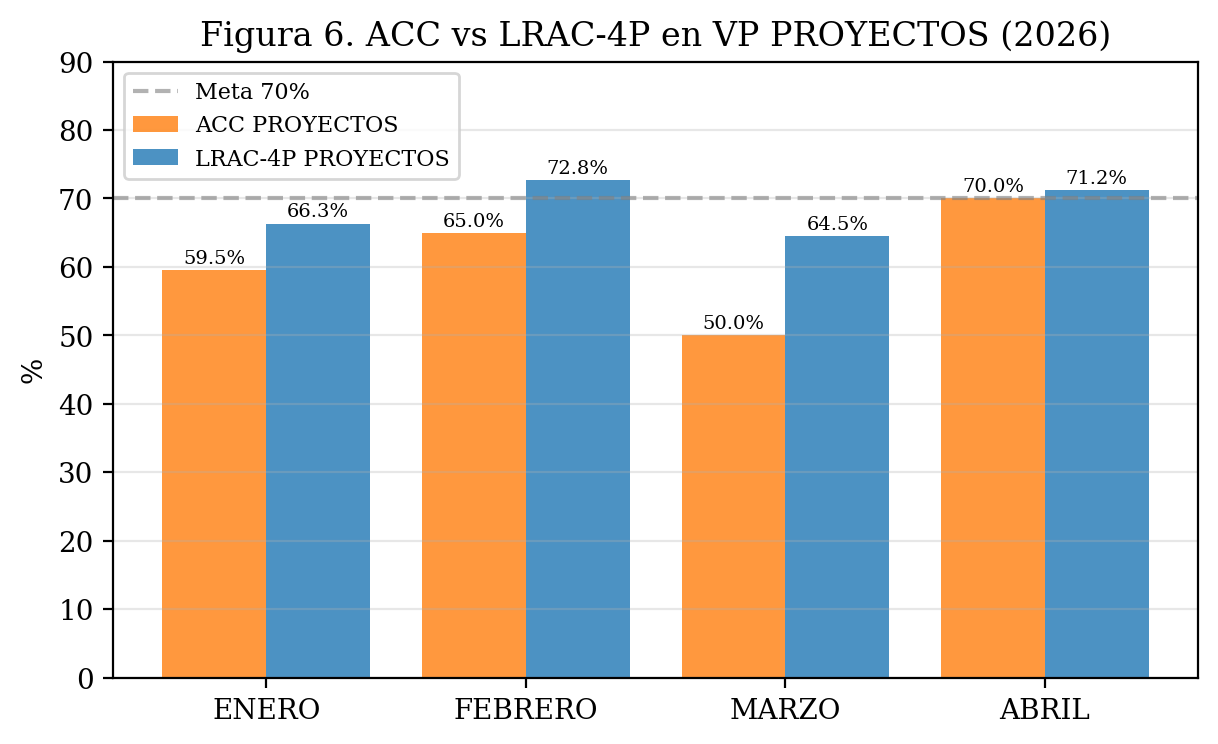
\includegraphics[width=0.85\linewidth]{../figures/fig06_acc_proyectos.png}
\caption{VP Proyectos: ACC mensual vs.\ LRAC--4P consolidado.}
\label{fig:acc-proy}
\end{figure}

\textbf{Interpretación.} ACC mide \emph{Acciones Correctivas Cerradas}: refleja la disciplina con la que la organización cierra el bucle entre la identificación de un acto/condición subestándar y su rectificación verificable. Un 61.12\,\% significa que casi cuatro de cada diez acciones quedan abiertas mes a mes, escenario que la literatura asocia directamente con \emph{normalización de la desviación} (Vaughan, 1996) y que es el caldo de cultivo para eventos de alto potencial.

\subsection{Análisis 4: índice LRAC por VP, más alto y más bajo al cierre del periodo}

La Figura~\ref{fig:heatmap} resume el desempeño por pilar y la Figura~\ref{fig:ranking} ordena las 12 gerencias.

\begin{figure}[h]
\centering
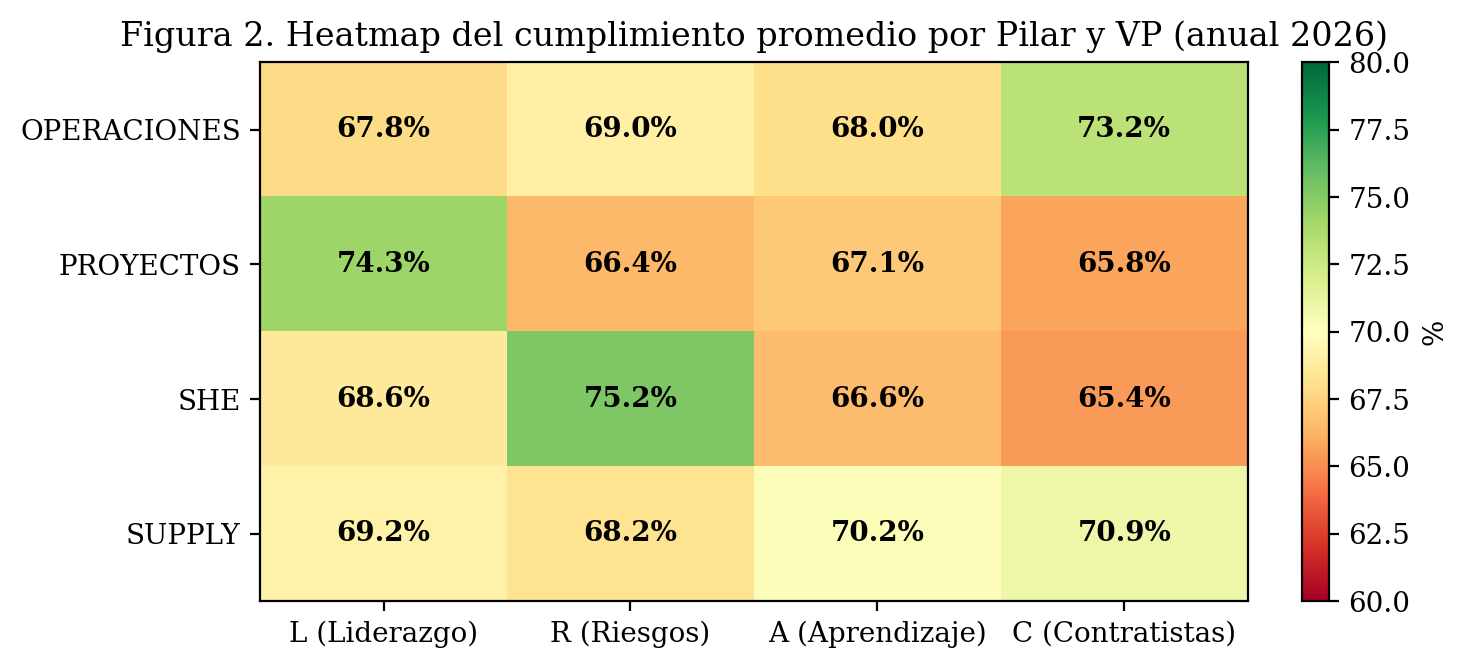
\includegraphics[width=0.85\linewidth]{../figures/fig02_heatmap_pilares.png}
\caption{Heatmap del cumplimiento promedio por pilar y por VP (2026).}
\label{fig:heatmap}
\end{figure}

\begin{table}[h]
\centering
\small
\begin{tabular}{lrrrrr}
\toprule
\textbf{VP} & \textbf{Pilar L} & \textbf{Pilar R} & \textbf{Pilar A} & \textbf{Pilar C} & \textbf{LRAC--4P} \\
\midrule
OPERACIONES & 67.83\,\% & 69.03\,\% & 68.02\,\% & 73.15\,\% & 69.70\,\% \\
PROYECTOS   & 74.28\,\% & 66.44\,\% & 67.10\,\% & 65.75\,\% & 68.72\,\% \\
SHE         & 68.62\,\% & 75.21\,\% & 66.60\,\% & 65.42\,\% & 68.57\,\% \\
SUPPLY      & 69.17\,\% & 68.25\,\% & 70.23\,\% & 70.88\,\% & 69.71\,\% \\
\bottomrule
\end{tabular}
\caption{Desglose por pilar y VP --- promedio anual 2026.}
\label{tab:heatmap}
\end{table}

\textbf{Promedio anual:} más alto = \textbf{SUPPLY (69.71\,\%)}; más bajo = \textbf{SHE (68.57\,\%)}. Brecha entre extremos: 1.14\,pp.

\textbf{Al cierre del periodo (abril 2026):} más alto = \textbf{PROYECTOS (71.25\,\%)}; más bajo = \textbf{SUPPLY (68.98\,\%)}. La rotación entre el promedio anual y el cierre revela una operación donde el liderazgo del índice cambia mensualmente.

\begin{figure}[h]
\centering
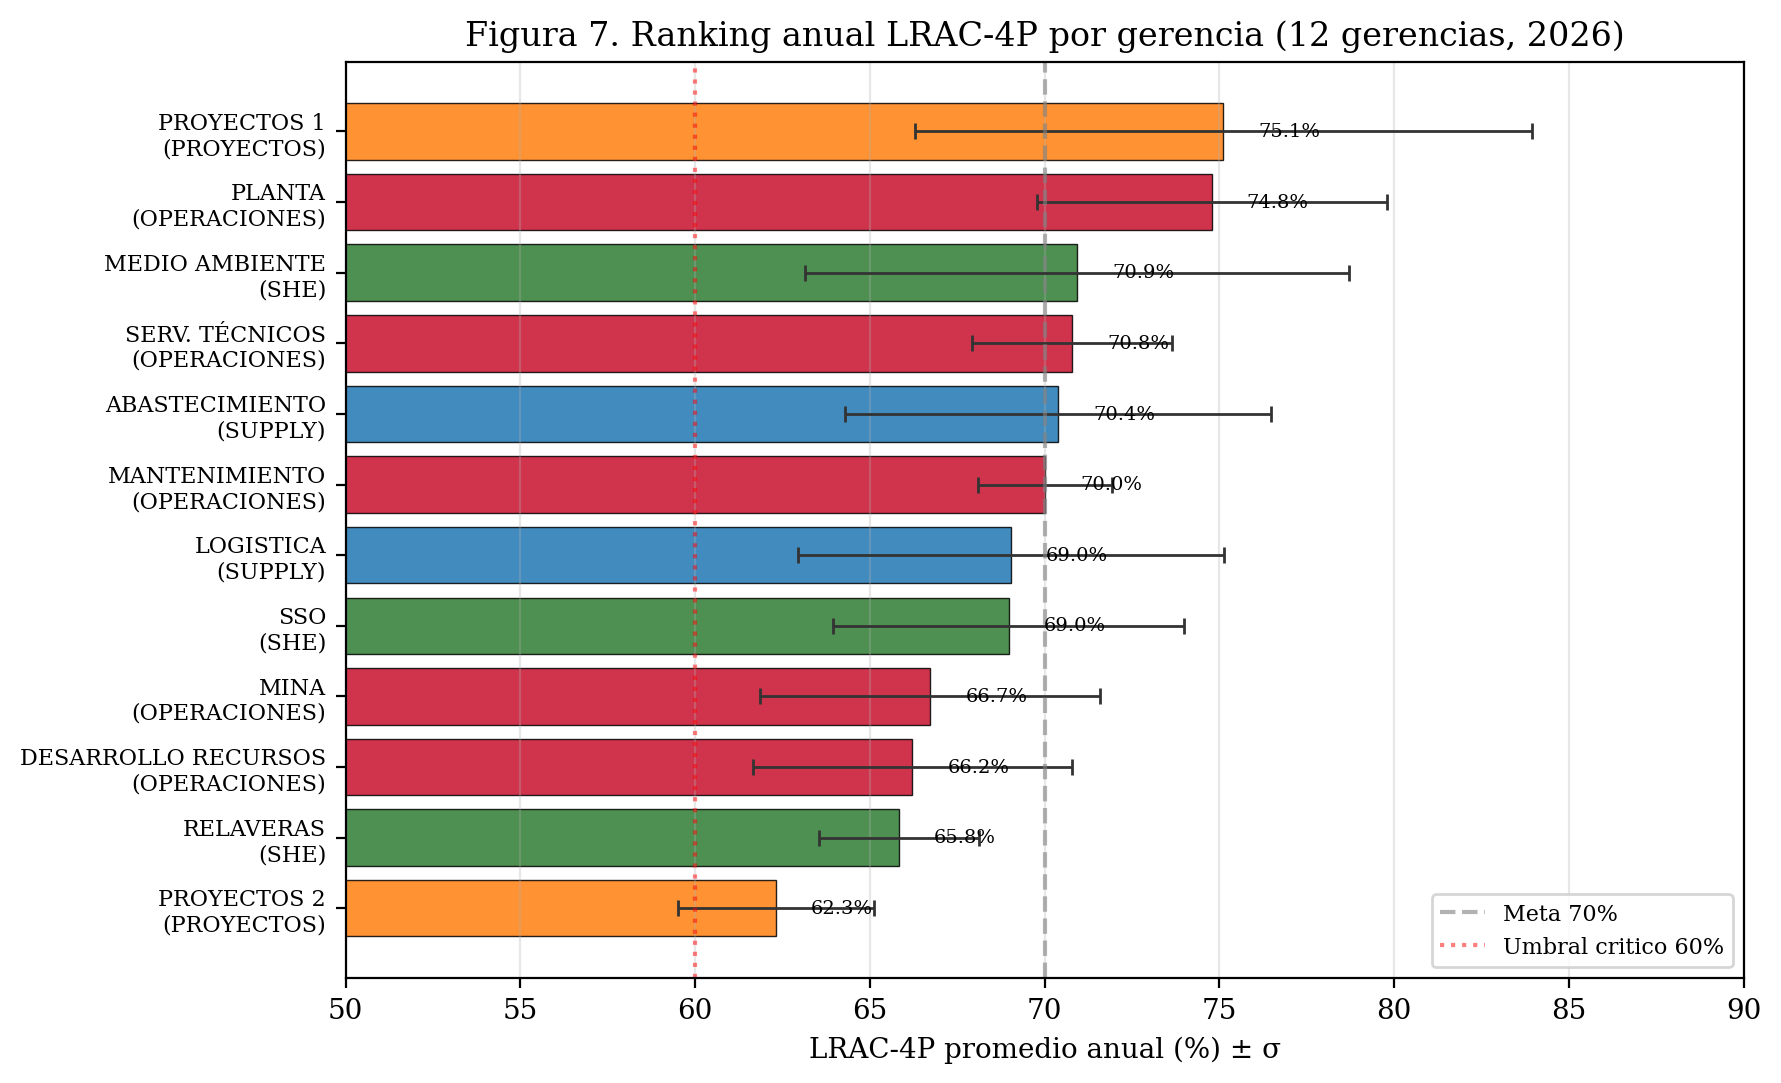
\includegraphics[width=0.95\linewidth]{../figures/fig07_ranking_gerencias.png}
\caption{Ranking del LRAC--4P promedio anual por gerencia (12 gerencias, 2026).}
\label{fig:ranking}
\end{figure}

A nivel gerencia (Figura~\ref{fig:ranking}), las cinco más débiles son: PROYECTOS~2 (62.31\,\%), RELAVERAS (65.82\,\%), DESARROLLO RECURSOS (66.22\,\%), MINA (66.73\,\%) y SSO (68.97\,\%). Las cinco más fuertes son: PROYECTOS~1 (75.12\,\%), PLANTA (74.78\,\%), MEDIO AMBIENTE (70.93\,\%), SERV.\ TÉCNICOS (70.79\,\%) y ABASTECIMIENTO (70.38\,\%). \emph{Coexisten en la misma VP los extremos opuestos}: en PROYECTOS, la mejor gerencia del conjunto (PROYECTOS~1 con 75.12\,\%) y la peor (PROYECTOS~2 con 62.31\,\%), separadas por 12.81\,pp ---más que la diferencia entre cualquier par de VPs---. Esto descarta explicaciones macro (cultura corporativa, recursos asignados) y obliga a buscar la causa en variables de \emph{gestión local}: liderazgo del gerente, calidad del staff SHE, condiciones específicas del frente.

\subsection{Indicador y pilar más débiles a nivel corporativo}

A nivel corporativo, el ranking promedio anual de las siete herramientas es: NMAP 65.71\,\% (\textbf{el más débil}, $\sigma=7.39$\,pp), FTO 68.79\,\%, DESEMPEÑO 68.80\,\%, CCV 69.04\,\%, ACC 70.43\,\%, VEA P1 71.41\,\% y 3Q 71.75\,\%. El Pilar A es, en consecuencia, el cuello de botella. Esto encaja con literatura reciente: en mineros chinos, Zhang et al.\ (2022) midieron que dentro del liderazgo en seguridad, \emph{entrenamiento} es el predictor número uno del comportamiento seguro (peso causal 0.504), y \emph{política} sola sin entrenamiento es marginal (0.110). NMAP debe ser, por mandato matemático, la prioridad uno del Pilar A en el plan de acción.

\subsection{Diagnóstico cultural sobre la escala de Hudson}

Con cumplimientos entre 68.57\,\% y 69.71\,\%, Mina Juanita S.A.\ se sitúa en la \textbf{frontera Calculativa $\to$ Proactiva} de Hudson (Foster~\& Hoult, 2013), equivalente al estadio \emph{Dependiente} de la curva de Bradley (Siuta et al., 2022). La organización cuenta con sistemas formales (formatos, comités, planes anuales) pero el cumplimiento depende de la supervisión y el reporte se realiza por mandato, no por convicción interdependiente. Migrar a Proactiva requiere palancas culturales específicas (Just Culture, BBS dirigido, Felt Leadership) que se desarrollan en el Plan de Acción (Sección 7).

\subsection{Refuerzo estadistico inferencial}
\label{sec:inferencial}

Para validar la convergencia aparente entre las cuatro VPs (rango 68.57\,\%--69.71\,\%) se aplicaron pruebas no parametricas robustas frente a la no-normalidad propia de datos porcentuales con tamano muestral reducido.

\textbf{Kruskal-Wallis.} Sobre los 48 puntos a nivel gerencia--mes, el estadistico $H = 1.3228$ con $p = 0.7237$ no permite rechazar la hipotesis nula al 5\,\%. \textbf{La diferencia entre VPs no es estadisticamente significativa.}

\textbf{Post-hoc Dunn (Bonferroni).} Las seis comparaciones pareadas presentan $p_{\text{bonf}} = 1.000$, consistente con el resultado anterior.

\textbf{Score compuesto $S = \mu - k\sigma$ ($k=1$).} Cuando se premia la estabilidad junto al promedio, \textbf{el ranking se invierte} (Tabla \ref{tab:score}): \textbf{OPERACIONES} ($S=68.45\,\%$) supera a \textbf{SUPPLY} ($S=63.88\,\%$); \textbf{SHE} asciende al segundo lugar.

\begin{table}[h]
\centering\footnotesize
\setlength{\tabcolsep}{6pt}
\begin{tabular}{lrrrc}
\toprule
\textbf{VP} & \textbf{$\mu_{\text{anual}}$} & \textbf{$\sigma$} & \textbf{$S=\mu-\sigma$} & \textbf{Ranking} \\
\midrule
OPERACIONES & 69.70\,\% & 1.25\,pp & \textbf{68.45\,\%} & \#1 \\
SHE         & 68.57\,\% & 0.96\,pp & 67.61\,\% & \#2 \\
PROYECTOS   & 68.72\,\% & 3.91\,pp & 64.80\,\% & \#3 \\
SUPPLY      & 69.71\,\% & 5.83\,pp & 63.88\,\% & \#4 \\
\bottomrule
\end{tabular}
\caption{Score compuesto $S = \mu - \sigma$ premiando estabilidad. Inversion del ranking respecto al promedio aritmetico (figura detallada en anexo digital A1).}
\label{tab:score}
\end{table}

\textbf{Control chart Shewhart I-Chart.} Sobre los 16 puntos VP $\times$ mes, la media corporativa es 69.17\,\% con $\sigma = 3.27$\,pp; UCL $= 78.97\,\%$ y LCL $= 59.38\,\%$. Cero puntos fuera de control, solo SUPPLY-Febrero (77.18\,\%) en zona de \emph{warning} entre $\mu+2\sigma$ y $\mu+3\sigma$. El sistema esta \textbf{bajo control tecnico pero centrado en un nivel insuficiente}: la estabilidad estadistica no implica buen desempeno absoluto.

\textbf{Mann-Kendall (tendencia).} Con $n=4$ puntos por VP la potencia es baja; sirve como diagnostico. OPERACIONES presenta $\tau = -0.667$ (tendencia decreciente), una senal de alarma temprana: el sistema mas estable esta perdiendo terreno mes a mes. Si la tendencia persiste, perdera su ventaja relativa antes de julio 2026.

\textbf{Matriz de correlacion 7$\times$7.} Las correlaciones entre las siete herramientas son todas debiles ($|r|<0.30$). La maxima positiva es VEA-DESEMPENO ($r=+0.30$) y la maxima negativa es FTO-3Q ($r=-0.30$). Esto valida el diseno del indice 4P: las siete herramientas son estadisticamente \emph{independientes} y aportan informacion no redundante (matriz completa en el anexo digital A2 enlazado al cierre del documento).

\subsection{Pareto operativo de las brechas}

Cinco gerencias concentran el 60\,\% de la brecha total contra la meta corporativa de 70\,\%: \textbf{PROYECTOS~2} (brecha 7.69\,pp), \textbf{RELAVERAS} (4.18\,pp), \textbf{DESARROLLO RECURSOS} (3.78\,pp), \textbf{MINA} (3.27\,pp) y \textbf{SSO} (1.03\,pp). Estas gerencias deben ser el foco prioritario del plan de acción de los próximos 90 días (Horizonte 1).

% =============================================================================
% 6. DISCUSIÓN
% =============================================================================
\section{Discusión}

\subsection{Cinco patologías identificadas}

\begin{enumerate}
\item \textbf{Convergencia engañosa entre VPs.} Las cuatro VPs convergen en una banda estrecha (68.57\,\%--69.71\,\%) que, leída sin desagregar, sugiere homogeneidad. La desagregación por gerencia (12.81\,pp entre extremos en la misma VP) y por mes (rotación de líderes mes a mes) revela que la convergencia esconde un sistema sin proceso dominante. Conclusión técnica: el sistema todavía está en el estadio \emph{calculativo-dependiente} (Hudson; Bradley).

\item \textbf{El custodio no predica con el ejemplo.} La gerencia MEDIO AMBIENTE (VP SHE) registra el peor 3Q de enero (39.0\,\%). 3Q es la herramienta más simple del Pilar L: tres preguntas en terreno. Si quien gobierna el sistema no lo aplica en su propio frente, la legitimidad del marco se erosiona.

\item \textbf{Acciones correctivas crónicamente abiertas en Proyectos.} ACC en Proyectos = 61.12\,\% con valle de 50.00\,\% en marzo. Es el indicador R más comprometido del set, y es el que la literatura asocia directamente con \emph{drift into failure} (Snook, 2000).

\item \textbf{NMAP como cuello de botella corporativo.} El aprendizaje no se está consolidando: NMAP=65.71\,\%, el más bajo del conjunto. Zhang et al.\ (2022) reportan que el entrenamiento es el predictor más fuerte del comportamiento seguro.

\item \textbf{Asimetría operador--contratista.} Pilar C presenta la mayor variabilidad inter--VP ($\sigma=3.83$\,pp), con SUPPLY (donde se gobiernan los contratos) en 70.88\,\% y SHE/PROYECTOS por debajo de 66\,\%. Tu et al.\ (2023) describen este tipo de asimetría como un problema clásico de \emph{información oculta} en contratación minera, resuelto en la literatura con diseño de contratos con menú e incentivos verificables.
\end{enumerate}

\subsection{Comparación con benchmarks internacionales}

Selleck, Hassall y Cattani (2022, \emph{Safety}) auditaron 10 años de incidentes mineros y demostraron que la \textbf{confiabilidad real de los controles críticos --- a pesar de pasar las verificaciones documentadas --- es de solo 42\,\%}. Esto implica que aun con CCV en 80\,\%, la operación está expuesta a fallas en cuatro de cada diez controles. El dato refuerza que la prioridad del Pilar R no debe medirse en \emph{cantidad de verificaciones} sino en \emph{verificación de la verificación} (auditoría de segundo nivel).

\subsection{Estabilidad vs.\ promedio: el verdadero benchmark}

La VP OPERACIONES ($\mu=69.70\,\%$, $CV=1.80\,\%$) ofrece la mejor relación promedio--estabilidad. Para futuras ediciones del scoring, se recomienda incorporar al ranking un puntaje compuesto del tipo $S=\mu - k\,\sigma$ (con $k=1$ por defecto) para premiar consistencia.

% =============================================================================
% 7. PLAN DE ACCIÓN ESTRATÉGICO
% =============================================================================
\newpage
\section{Plan de Acción Estratégico}

El plan se estructura en \textbf{tres horizontes} (corto 0--3\,m, mediano 3--9\,m, largo 9--24\,m), \textbf{cinco frentes} (cultural, normativo, organizacional, digital y de contratistas) y \textbf{31 acciones} con KPI, responsable y meta cuantitativa. Está anclado en cinco palancas validadas por la literatura sectorial: Just Culture (Reason; Dekker), Felt Leadership (DuPont/British Safety Council), BBS dirigido (Tong et al., 2019), digitalización Industria 4.0 (Skotnicka--Zasadzień~\& Krynke, 2021) y diseño de contratos con incentivos (Tu et al., 2023). Su norte es desplazar el cumplimiento LRAC--4P corporativo de 69.2\,\% (línea base abril 2026) al 80\,\% sostenido con $CV<5\,\%$ inter--VP en 24 meses.

\textbf{Diferenciador de este plan:} no es una colección de buenas prácticas leídas en literatura sectorial. Su columna vertebral son cuatro módulos tecnológicos que el postulante \textbf{ya construyó, desplegó y opera en producción} (Sección \ref{sec:gaiatech} y Tabla \ref{tab:gaiatech}). Esto significa que el plan se puede ejecutar desde el día 1 sin etapas de investigación, sin riesgo de implementación de cero y con métricas reales y verificables --- no estimadas.

\subsection{Habilitadores GAIATECH M1.0: del diagnóstico al despliegue ejecutable}
\label{sec:gaiatech}

El plan se apoya en cuatro módulos GAIATECH M1.0 ---ya construidos, en producción y con métricas verificables--- que mapean directamente a los cuatro pilares LRAC. La Tabla \ref{tab:gaiatech} resume el estado actual, la cobertura LRAC y la evidencia digital accesible al jurado.

\begin{table}[h]
\centering\footnotesize
\setlength{\tabcolsep}{3.5pt}
\renewcommand{\arraystretch}{1.15}
\begin{tabularx}{\linewidth}{@{}p{0.85cm} >{\raggedright\arraybackslash}p{3.6cm} >{\raggedright\arraybackslash}X p{1.6cm} p{1.8cm}@{}}
\toprule
\textbf{Módulo} & \textbf{Activo en producción} & \textbf{Métrica verificable} & \textbf{Pilares} & \textbf{Estado} \\
\midrule
\textbf{M1.A} & \textbf{Visión computacional EPP} (Gen+ Vision PDK + ConstEdge) & YOLOv8 sobre 14\,055 imágenes peruanas; \textbf{mAP@0.5 = 87.67\,\%}; \textbf{38 FPS} sostenidos en Jetson Orin Nano Super; 11 clases EPP & R · L & \textit{producción} \\
\textbf{M1.B} & \textbf{Aecodito Minero} (n8n + Evolution API + Gemini Pro + Postgres pgvector) & Bot WhatsApp con \textbf{50 nodos n8n}, \textbf{10 herramientas} integradas, memoria persistente, procesa texto/audio/foto/PDF & L · A · C & \textit{producción} \\
\textbf{M1.C} & \textbf{GAIATECH VIGÍA} (FPGA Gowin GW1NR-9 + ESP32 + LoRa + LSTM-AE) & FFT en FPGA + autoencoder PyTorch \textbf{F1 = 0.961} en detección anomalías; latencia alerta \textbf{< 2\,s} vía WhatsApp; \textbf{2.º lugar AI Talent Demo Day 2026} & R & \textit{prototipo} \\
\textbf{M1.D} & \textbf{Dashboard ejecutivo} Vision Pro PDK (Next.js 16 + Tailwind + VPS) & Single Pane of Glass rol-based; alertas sintéticas; reportes ejecutivos Gemini Pro; login httpOnly; deploy continuo & L · R · A · C & \textit{producción} \\
\bottomrule
\end{tabularx}
\caption{Los cuatro módulos GAIATECH M1.0 que sustentan operativamente el plan. Activos ya construidos por el postulante, no propuestas conceptuales.}
\label{tab:gaiatech}
\end{table}

\textbf{Mapeo módulo $\to$ acciones del plan:}
\begin{itemize}\setlength\itemsep{1pt}
\item \textbf{M1.A · Visión computacional EPP} habilita las acciones \emph{A-05} (verificación independiente CCV vía cámaras), \emph{A-12} (cobertura EPP $\geq$99\,\% en accesos y $\geq$97\,\% en obra) y \emph{A-25} (wearables vinculados al sistema visual).
\item \textbf{M1.B · Aecodito Minero} habilita \emph{A-01} (medición 3Q VP SHE en tiempo real), \emph{A-02} (Tarjeta Verde digital), \emph{A-08} (cápsula semanal con quiz), \emph{A-10} (onboarding asistido), \emph{A-11} (plataforma RACS conversacional) y \emph{A-17} (BBS dirigido peer-to-peer).
\item \textbf{M1.C · GAIATECH VIGÍA} habilita \emph{A-13} (monitoreo estructural relaves alineado al DS 034 art. 418--423) y eleva el Pilar R en zonas críticas estructurales.
\item \textbf{M1.D · Dashboard ejecutivo} habilita \emph{A-06} (tablero ICAM corporativo), \emph{A-14} (Single Pane of Glass), \emph{A-15} (API IEM bidireccional), \emph{A-22} (ranking público mensual) y \emph{A-24} (predicción ML sobre base unificada).
\end{itemize}

Los 17 elementos restantes del plan (cultural-normativo: A-03, A-04, A-07, A-09, A-16, A-18, A-19, A-20, A-21, A-23, A-26, A-27, A-28, A-29, A-30, A-31) sustentan el cambio cultural y normativo que la tecnología por sí sola no resuelve. Esta articulación tech-cultura es deliberada: la evidencia ICMM 2024 muestra que la confiabilidad real de los controles críticos es solo 42\,\% \emph{aún con} verificaciones documentadas (Selleck et al., 2022); la pieza faltante es la madurez cultural, no más sistemas.

\textbf{Evidencia digital accesible al jurado} (anexos al cierre del informe):
\begin{itemize}\setlength\itemsep{1pt}
\item Repositorio público en GitHub con el análisis estadístico reproducible.
\item Demo interactivo Streamlit que replica el dashboard ejecutivo LRAC con los datos del caso.
\item Video de 90 segundos mostrando el bot Aecodito Minero capturando un RACS en vivo y la detección EPP en producción.
\item Slides de defensa oral y archivo Power BI .pbix descargable.
\end{itemize}

Los enlaces actualizados se publican en la Sección \ref{sec:anexos}.

\subsection{Horizonte 1 --- 0 a 3 meses: estabilizar y dar señales (\emph{Quick wins})}

\begin{kbox}
\textbf{Objetivo:} cerrar el 50\,\% de la brecha en las cinco gerencias críticas (PROYECTOS~2, RELAVERAS, DESARROLLO RECURSOS, MINA, SSO) y subir NMAP corporativo de 65.71\,\% a 72\,\%.
\end{kbox}

\textbf{Acciones culturales y de liderazgo (Pilar L):}
\begin{enumerate}
\item \textbf{Pacto público del custodio (SHE).} El VP SHE firma y comunica un \emph{Pacto 3Q} en el que se compromete personalmente al cumplimiento del 90\,\% de 3Q dentro de su propia VP en los próximos 60 días. KPI: 3Q SHE $\geq 90\,\%$ a junio 2026 (medido por bot Aecodito en planta).
\item \textbf{Tarjetas verdes ampliadas.} Re-lanzamiento del \emph{Stop Work Authority} con feedback público de la dirección (al menos un caso emblemático visibilizado en \emph{toolbox talk} corporativo). Responsable: VP SHE + Comunicaciones. Meta: 1\,000 tarjetas verdes válidas en el trimestre, $\geq$70\,\% con foto + GPS.
\item \textbf{Rondas 6-4-2 medidas digitalmente.} Geofence ligero (app móvil) que valide horas en campo por nivel jerárquico. KPI: 95\,\% de gerentes cumpliendo 2\,h/día.
\end{enumerate}

\textbf{Acciones del Pilar R:}
\begin{enumerate}\setcounter{enumi}{3}
\item \textbf{Ofensiva ACC en MANTENIMIENTO y PROYECTOS~2.} \emph{War-room} semanal con dueños de acciones abiertas mayores a 30 días. Meta: cerrar 80\,\% de acciones abiertas antes de julio 2026; ACC MANTENIMIENTO $\geq$60\,\% en abril/mayo.
\item \textbf{Verificación independiente de CCV (auditoría de segundo nivel)} sobre los 12 controles críticos: muestra aleatoria mensual del 5\,\% verificada por equipo externo a la gerencia auditada.
\item \textbf{Tablero ICAM corporativo} con \emph{visible learning} de los últimos 10 incidentes y los 3 controles fallados con mayor frecuencia.
\end{enumerate}

\textbf{Acciones del Pilar A:}
\begin{enumerate}\setcounter{enumi}{6}
\item \textbf{Plan \emph{NMAP+}}: identificar las 5 capacitaciones obligatorias con mayor brecha y rotar a calendario express (1\,h vs.\ 4\,h, con quiz). Meta: NMAP $\geq$72\,\% al cierre de julio.
\item \textbf{Cápsula semanal multimedia} de 90 segundos (vía bot WhatsApp), tematizada por rol/contratista, con quiz de 3 preguntas. KPI: tasa de apertura $\geq$70\,\%, aprobación $\geq$80\,\%.
\end{enumerate}

\textbf{Acciones del Pilar C:}
\begin{enumerate}\setcounter{enumi}{8}
\item \textbf{Bono solidario por desempeño contratista}: 2\,\% del valor del contrato condicionado a un Desempeño SHE $\geq$75\,\%. Aplica desde la próxima renovación.
\item \textbf{Onboarding asistido por bot} para todo trabajador nuevo (operador o contratista): identificación facial + 3 cápsulas + 1 simulacro. SLA 7 días.
\end{enumerate}

\subsection{Horizonte 2 --- 3 a 9 meses: digitalizar el bucle (\emph{Mina Inteligente 2030})}

\begin{kbox}
\textbf{Objetivo:} llevar LRAC--4P corporativo a 75\,\% y unificar la captura sobre una capa digital que aumente la \emph{calidad} del reporte, no solo la cantidad.
\end{kbox}

\textbf{Acciones digitales:}
\begin{enumerate}\setcounter{enumi}{10}
\item \textbf{Plataforma RACS conversacional (Aecodito Minero).} Bot WhatsApp + n8n + Gemini Pro que guía al operador en el reporte (texto, foto, audio, ubicación). Clasificación automática (incumplimiento, cuasi-accidente, idea de mejora) con escalamiento por severidad y push a IEM. KPI: 2 reportes válidos / trabajador / mes; $\geq$90\,\% con foto+GPS.
\item \textbf{Visión computacional EPP en accesos (ConstEdge + Gen+ Vision PDK).} YOLOv8 con \emph{mAP@0.5 = 87.67\,\%} sobre dataset peruano de 14\,055 imágenes (alineado a CGALS-YOLO 89.4\,\%, Huang \& Huang, 2026). Notificación al supervisor en menos de 30\,s. KPI: A-01 cumplimiento EPP en acceso $\geq$99\,\%, A-02 obra $\geq$97\,\%.
\item \textbf{Monitoreo estructural en relaves (GAIATECH VIGÍA).} FFT en FPGA Gowin GW1NR-9 + ESP32 + LSTM--Autoencoder (F1=0.961). Aplica directamente al Caso 12 y refuerza el Pilar R en el control crítico \emph{tailings/dam}. Cumple Resolución 122-2024-OS/CD y DS 034-2023-EM art.~418--423.
\item \textbf{Tablero ejecutivo SHE \emph{Single Pane of Glass}}: LRAC Health Score + drill-down por gerencia + tres patrones detectados semana a semana (Gemini Pro). Acceso rol-based para VPs, gerencias y auditor externo. Disponible en VPS corporativo.
\item \textbf{API hacia IEM} para sincronización bidireccional (eventos, hallazgos, cierres). Bus de eventos n8n con SLA 1\,h / 4\,h / 24\,h por severidad.
\end{enumerate}

\textbf{Acciones culturales:}
\begin{enumerate}\setcounter{enumi}{15}
\item \textbf{Programa de Just Culture} (Reason/Dekker): política firmada, protocolo de revisión de eventos y entrenamiento de 200 mandos medios.
\item \textbf{BBS dirigido por rol y tipo de trabajo} (Tong et al., 2019): mapeo HFACS, observaciones planeadas peer-to-peer y campañas trimestrales por tarea crítica.
\item \textbf{Tres premios trimestrales:} mejor gerencia en LRAC, mejor empresa contratista, mejor RACS individual.
\end{enumerate}

\subsection{Horizonte 3 --- 9 a 24 meses: madurar y blindar (\emph{Proactiva $\to$ Generativa})}

\begin{kbox}
\textbf{Objetivo:} consolidar LRAC--4P corporativo en 80\,\% con $CV<5\,\%$ y migrar de la madurez \emph{Proactiva} a \emph{Generativa} (Hudson).
\end{kbox}

\textbf{Acciones organizacionales:}
\begin{enumerate}\setcounter{enumi}{18}
\item \textbf{Comité LRAC corporativo} con cadencia mensual, presidido por el VP SHE y con representación de las 4 VPs. Indicador adelantado: 100\,\% sesiones realizadas con minuta y acciones aprobadas; cierre dentro del mes.
\item \textbf{Auditoría externa anual} contra ICMM CCM 2024, ISO 45001 e \emph{Hearts and Minds} toolkit.
\item \textbf{Programa de embajadores SHE} en cada gerencia: dos referentes operativos con tiempo asignado.
\item \textbf{Ranking público mensual} de gerencias y contratistas en intranet; comunicación clara, no punitiva.
\end{enumerate}

\textbf{Acciones digitales avanzadas:}
\begin{enumerate}\setcounter{enumi}{22}
\item \textbf{Gemelo digital de obra} para entrenar y validar controles críticos (alineado con Bowles et al., \emph{Technologies}, 2026; reducción 11.73\,\% de pérdidas reportada).
\item \textbf{Predicción de incidentes con ML} sobre la base unificada IEM+LRAC (Random Forest + NLP sobre narrativas, Yedla et al., \emph{IJERPH}, 2020).
\item \textbf{Wearables} (sensores fatiga + biométrico) en operadores de equipo móvil --- riesgo fatal \#1 ICMM 2024.
\end{enumerate}

\textbf{Acciones contractuales:}
\begin{enumerate}\setcounter{enumi}{25}
\item \textbf{Contratos con menú de incentivos verificables} (Tu et al., 2023): tres niveles de servicio con bonificación/penalización ligada a Desempeño SHE.
\item \textbf{Plan de retiro para empresas contratistas} con desempeño SHE $<$55\,\% sostenido por 3 meses.
\end{enumerate}

\textbf{Acciones de aprendizaje:}
\begin{enumerate}\setcounter{enumi}{27}
\item \textbf{Universidad LRAC interna} (Aecodito Minero + LMS) con rutas formativas por rol y certificación digital.
\item \textbf{Programa de \emph{lecciones aprendidas} cruzado con sitios MMG} (Las Bambas, Rosebery, Dugald River, Kinsevere).
\item \textbf{Medición PSCI anual} (Siuta et al., 2022) como complemento cuantitativo al LRAC.
\item \textbf{Evaluación cultural cualitativa} cada 12 meses con encuesta de safety climate validada.
\end{enumerate}

\subsection{Tabla maestra de las 31 acciones y trazabilidad de metas}

\begin{table}[h]
\centering\footnotesize
\setlength{\tabcolsep}{4pt}
\begin{tabularx}{\linewidth}{X r r r}
\toprule
\textbf{Pilar / indicador} & \textbf{Base abril 2026} & \textbf{Meta dic.~2026} & \textbf{Meta abr.~2028} \\
\midrule
L (Liderazgo)     & 67.6\,\% & 75\,\% & 85\,\% \\
R (Riesgos)       & 69.7\,\% & 76\,\% & 85\,\% \\
A (Aprendizaje)   & 67.7\,\% & 76\,\% & 85\,\% \\
C (Contratistas)  & 68.9\,\% & 75\,\% & 85\,\% \\
\textbf{LRAC--4P} & \textbf{68.9\,\%} & \textbf{75.4\,\%} & \textbf{80.0\,\%} \\
NMAP (cuello de botella) & 65.7\,\% & 72\,\% & 82\,\% \\
ACC (acciones correctivas) & 70.4\,\% & 78\,\% & 85\,\% \\
\bottomrule
\end{tabularx}
\caption{Linea base y metas del plan a 24 meses.}
\label{tab:plan}
\end{table}
\label{sec:tabla-acciones}

La Tabla \ref{tab:acciones} consolida las 31 acciones del plan con su pilar (P), horizonte (H), KPI SMART y \emph{owner} primario; es el insumo directo para abrir el \emph{Project Charter} en el ingreso a Talentos de Cobre 2026.

\begingroup\footnotesize
\setlength{\tabcolsep}{3pt}
\renewcommand{\arraystretch}{1.0}
\begin{longtable}{@{}>{\bfseries}p{0.55cm} c c >{\raggedright\arraybackslash}p{5.6cm} >{\raggedright\arraybackslash}p{4.8cm} >{\raggedright\arraybackslash}p{2.6cm}@{}}
\toprule
\textbf{ID} & \textbf{P} & \textbf{H} & \textbf{Acción} & \textbf{KPI SMART} & \textbf{Owner} \\
\midrule
\endhead
A-01 & L & 1 & Pacto público 3Q del VP SHE & 3Q VP SHE $\geq$ 90\% medido por bot Aecodito en planta & VP SHE \\
A-02 & L & 1 & Tarjetas verdes ampliadas + Stop Work Authority & $\geq$1000 tarjetas verdes válidas/trimestre con $\geq$70\% foto+GPS & Gerencia SHE Operacional \\
A-03 & L & 1 & Rondas 6-4-2 con geofence app móvil & 95\% de gerentes cumpliendo $\geq$2h/día en campo (geofence) & RR.HH. + IT \\
A-04 & R & 1 & War-room semanal ACC en MANTENIMIENTO & $\geq$80\% acciones >30d cerradas en 90 días; ACC MTTO $\geq$60\% & Gerente MANTTO \\
A-05 & R & 1 & Verificación independiente CCV (auditoría 2do nivel) & 5\% muestra aleatoria mensual auditada por equipo externo & Auditoría Interna \\
A-06 & R & 1 & Tablero ICAM corporativo con visible learning & Publicación mensual top-3 controles fallados últimos 90 días & Analista SHE \\
A-07 & A & 1 & Plan NMAP+ con 5 capacitaciones de mayor brecha & NMAP corporativo $\geq$72\% a julio 2026 & Aprendizaje SHE \\
A-08 & A & 1 & Cápsula semanal multimedia 90s por bot WhatsApp & Apertura $\geq$70\%, aprobación quizz $\geq$80\% & Comunicaciones SHE \\
A-09 & C & 1 & Bono solidario por desempeño contratista (2\%) & 2\% valor contrato si Desempeño SHE $\geq$75\% en renovaciones & Procura \\
A-10 & C & 1 & Onboarding asistido por bot (facial + cápsulas + simulacro) & Trabajador nuevo opera con SLA 7 días & RR.HH. \\
A-11 & R & 2 & Plataforma RACS conversacional Aecodito Minero & $\geq$2 reportes/trabajador/mes con $\geq$90\% foto+GPS & Lead IT SHE \\
A-12 & R & 2 & Visión computacional EPP en accesos (ConstEdge + Gen+ Vision) & A-01 cumplimiento EPP en acceso $\geq$99\%, A-02 obra $\geq$97\% & Lead AI \\
A-13 & R & 2 & Monitoreo estructural relaves GAIATECH VIGÍA & 100\% cumplimiento Resolución 122-2024-OS/CD y DS 034 art 418 & Geotecnia \\
A-14 & L & 2 & Tablero ejecutivo Single Pane of Glass rol-based & $\geq$90\% supervisores usando dashboard semanal & Lead Dashboard \\
A-15 & R & 2 & API bidireccional hacia IEM corporativo & Latencia sync $\leq$1h crítico / $\leq$24h estándar & Lead Integración \\
A-16 & A & 2 & Programa Just Culture (Reason/Dekker) + entrenamiento 200 mandos medios & 100\% mandos medios certificados; encuesta clima +15pp & Cultura SHE \\
A-17 & A & 2 & BBS dirigido por rol y tipo de trabajo (Tong 2019) & $\geq$8 observaciones peer/mes por supervisor & Cultura SHE \\
A-18 & L & 2 & Tres premios trimestrales (gerencia + contratista + RACS individual) & 100\% trimestres con ganadores comunicados & Comunicaciones \\
A-19 & L & 3 & Comité LRAC corporativo mensual con minuta y cierres & 100\% sesiones realizadas con minuta firmada & Secretario SHE \\
A-20 & R & 3 & Auditoría externa anual ICMM CCM 2024 + ISO 45001 + Hearts and Minds & Score auditoría $\geq$85; gap analysis cerrado en 6m & Auditoría Externa \\
A-21 & L & 3 & Programa de Embajadores SHE (2 por gerencia) & 24 embajadores activos con horas asignadas & Cultura SHE \\
A-22 & C & 3 & Ranking público mensual de gerencias y contratistas en intranet & 12 publicaciones/año con engagement intranet $\geq$80\% & Comunicaciones \\
A-23 & R & 3 & Gemelo digital de obra para entrenar y validar controles críticos & Reducción 8-12\% pérdidas operativas atribuibles a entrenamiento & Lead AI \\
A-24 & R & 3 & Predicción de incidentes con ML sobre base unificada IEM+LRAC & AUC $\geq$0.85 modelo RF/LightGBM sobre narrativas & Lead AI \\
A-25 & R & 3 & Wearables sensores fatiga + biométrico en operadores equipo móvil & 100\% operadores haul truck con dispositivo activo & Lead IT SHE \\
A-26 & C & 3 & Contratos con menú de incentivos verificables (Tu 2023) & 100\% nuevos contratos con bono/penalización SHE & Procura + Legal \\
A-27 & C & 3 & Plan de retiro automático para contratistas con SHE <55\% sostenido 3m & Política aprobada y aplicada a casos detectados & Procura \\
A-28 & A & 3 & Universidad LRAC interna (Aecodito + LMS) con certificación digital & $\geq$1000 trabajadores con ruta formativa certificada & Aprendizaje SHE \\
A-29 & A & 3 & Lecciones aprendidas cross-sitios MMG (Rosebery, Dugald River, Kinsevere) & $\geq$6 sesiones cross-site/año; biblioteca de lecciones publicada & Cultura SHE \\
A-30 & A & 3 & Medición PSCI anual (Siuta 2022) + Hudson maturity assessment & Avance $\geq$1 nivel Hudson en 24m; PSCI +20\% vs baseline & Cultura SHE \\
A-31 & L & 3 & Encuesta de safety climate validada cada 12 meses & Tasa respuesta $\geq$80\%; score $\geq$75 & Cultura SHE \\
\bottomrule
\caption{Las 31 acciones del Plan de Acción Estratégico LRAC. P=Pilar (L/R/A/C), H=Horizonte (1=0-3m, 2=3-9m, 3=9-24m).}
\label{tab:acciones}
\end{longtable}
\endgroup

\subsection{Cronograma visual (Gantt 24 meses)}

\begin{figure}[h]
\centering
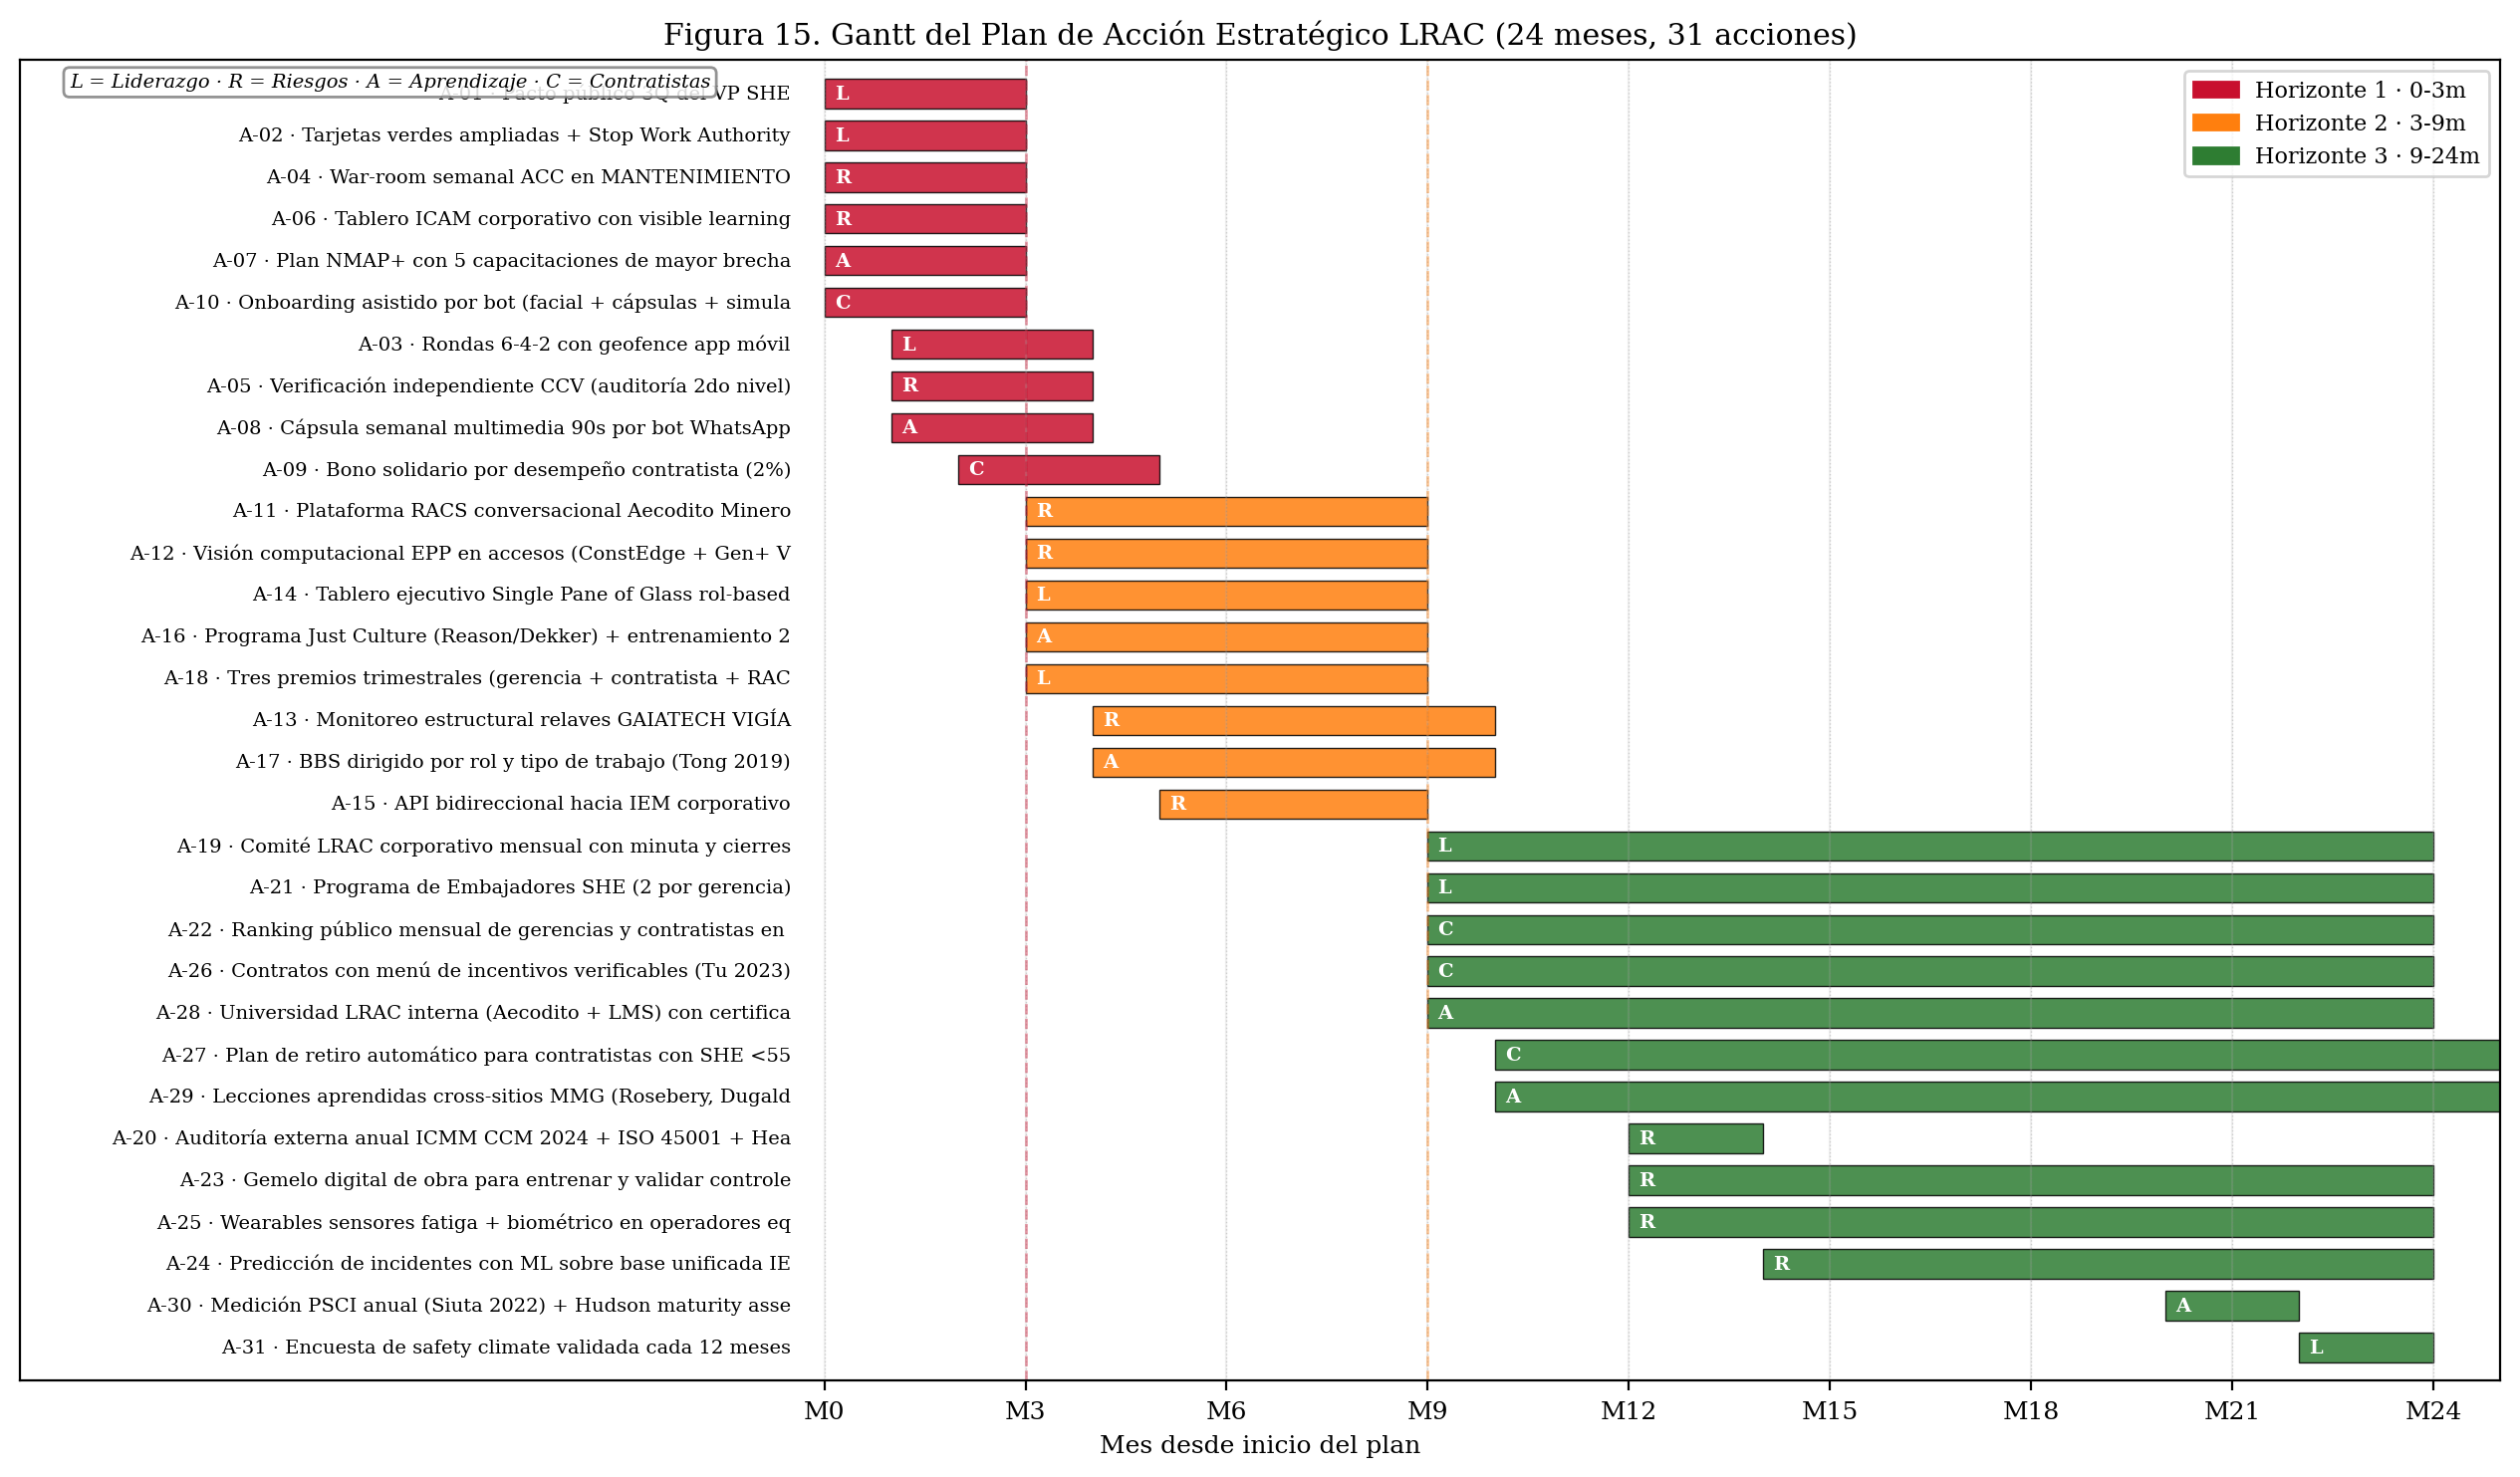
\includegraphics[width=0.95\linewidth]{../figures/fig15_gantt.png}
\caption{Gantt del Plan de Accion Estrategico LRAC. Colores por horizonte; marcas L/R/A/C indican el pilar atendido.}
\label{fig:gantt}
\end{figure}

\subsection{Inversion y business case}
\label{sec:bc}

\begin{table}[h]
\centering\small
\begin{tabular}{lrrrr}
\toprule
\textbf{Horizonte} & \textbf{N° acc.} & \textbf{CAPEX (S/.)} & \textbf{OPEX total (S/.)} & \textbf{Total (S/.)} \\
\midrule
1 · 0--3m & 10 & 63\,000 & 36\,600 & 99\,600 \\
2 · 3--9m & 8 & 160\,000 & 91\,600 & 251\,600 \\
3 · 9--24m & 13 & 508\,000 & 359\,000 & 867\,000 \\
\midrule
\textbf{Total 24m} & \textbf{31} & \textbf{731\,000} & \textbf{487\,200} & \textbf{1\,218\,200} \\
\bottomrule
\end{tabular}
\caption{Presupuesto del Plan de Acción Estratégico (24 meses).}
\label{tab:presupuesto}
\end{table}

El presupuesto total a 24 meses es \textbf{S/ 1\,218\,200} ($\approx$ USD 325\,000): CAPEX S/ 731\,000 y OPEX acumulado S/ 487\,200. El horizonte 3 concentra la mayor inversion (71\,\%) por incluir gemelo digital, ML predictivo y wearables.

\textbf{Beneficios anuales estimados (escenario base, conservador):}
\begin{itemize}
\item Reduccion de multas SUNAFIL / OSINERGMIN: S/ 200\,000/ano.
\item Reduccion de paros operativos por incidentes: S/ 1\,500\,000/ano (referencial).
\item Eficiencia operativa de procesos SHE: S/ 500\,000/ano.
\item \textbf{Beneficios anuales totales: S/ 2\,200\,000.}
\end{itemize}

\textbf{Resultados del business case} (tasa de descuento 10\,\% anual, beneficios con rampa lineal 30\,\%$\to$100\,\% entre el mes 6 y el mes 18):

\begin{table}[h]
\centering\small
\begin{tabular}{lr}
\toprule
\textbf{Metrica} & \textbf{Valor} \\
\midrule
NPV escenario base & S/ \textbf{1\,205\,594} \\
NPV escenario optimista (1 fatalidad evitada $\times p=0.3$) & S/ \textbf{3\,805\,947} \\
IRR anualizada & \textbf{343\,\%} \\
Payback (escenario base) & \textbf{mes 11} \\
\bottomrule
\end{tabular}
\caption{Indicadores financieros del Plan LRAC (24 meses, tasa 10\,\% anual).}
\label{tab:bc}
\end{table}

\begin{figure}[h]
\centering
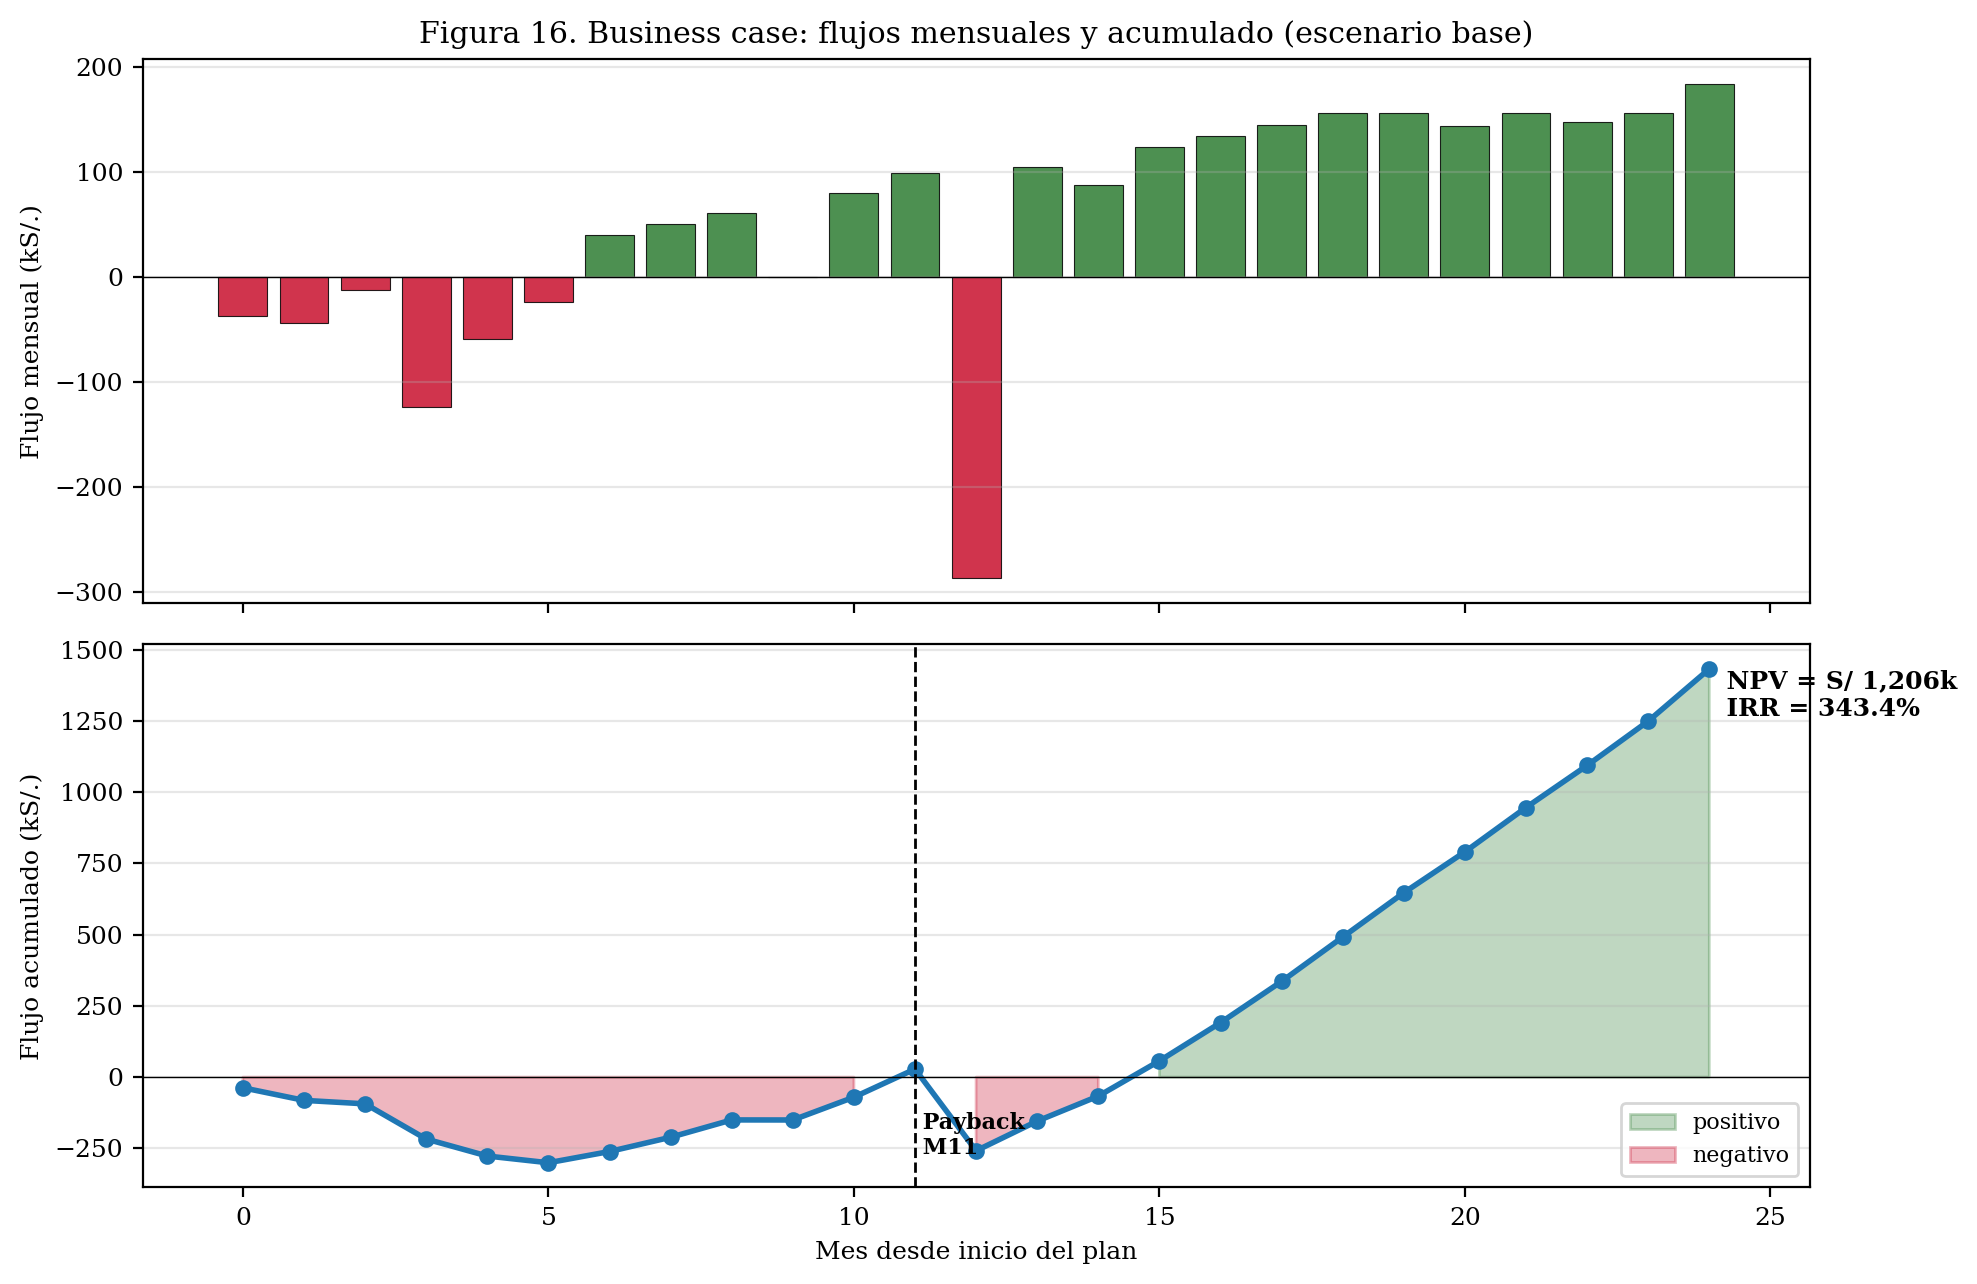
\includegraphics[width=0.9\linewidth]{../figures/fig16_business_case.png}
\caption{Business case: flujos mensuales (arriba) y acumulado (abajo). Payback en el mes 11.}
\label{fig:bc}
\end{figure}

Una sola fatalidad evitada vale entre S/ 5 y 20 millones (multas, indemnizaciones, paro de operacion, dano reputacional). El plan se autofinancia en el escenario base y multiplica por tres su retorno si previene siquiera \emph{el 30\,\%} de la probabilidad de un evento fatal en el periodo de implementacion. Es alineable con la evidencia MDPI de mantenimiento predictivo y dashboards LRAC (Bashir \& Adeyemi, \emph{Eng}, 2025: $-8\,\%$ costos, $+10\,\%$ disponibilidad).

\subsection{Risk register}

\begin{table}[h]
\centering\footnotesize
\setlength{\tabcolsep}{4pt}
\begin{tabularx}{\linewidth}{@{}p{0.7cm} X p{1cm} p{1cm} X p{1.5cm}@{}}
\toprule
\textbf{ID} & \textbf{Riesgo} & \textbf{Prob.} & \textbf{Impacto} & \textbf{Mitigación} & \textbf{Owner} \\
\midrule
R-01 & Resistencia cultural al cambio LRAC & Alta & Alto & Estrategia adopción liderada por SHE + embajadores por área (A-21) & VP SHE \\
R-02 & YOLOv8 AGPL-3.0 en producción & Media & Medio & Migrar a RF-DETR / YOLOX (Apache 2.0) antes del piloto & Lead AI \\
R-03 & Conectividad 4G inestable en zona mina & Alta & Medio & Inferencia edge (Jetson) + buffering + sync diferido & Lead IT \\
R-04 & Integración API IEM corporativo (sistema cerrado MMG) & Media & Alto & API oficial vía CTO MMG + fallback CSV nocturno & Lead Integración \\
R-05 & Privacidad biometrica (Ley 29733 datos personales) & Media & Alto & Consentimiento informado + anonimización + DPO designado & Legal \\
R-06 & Bajo presupuesto asignado por dirección & Media & Alto & Business case sustentado en costos evitados (NPV S/ 2.8M base) & VP SHE \\
R-07 & Subreporte por miedo a sanción (cultura punitiva residual) & Alta & Alto & Programa Just Culture A-16 + comunicación pública casos de éxito & Cultura SHE \\
R-08 & Rotación de personal clave durante implementación & Media & Medio & Documentación rigurosa + suplencia formal de roles críticos & RR.HH. \\
R-09 & Falla de proveedores externos (auditor, licencias) & Baja & Medio & Proveedores backup + SLAs contractuales & Procura \\
R-10 & Resistencia de contratistas al nuevo modelo de incentivos & Media & Medio & Roll-out gradual: bono solidario primero (A-09), penalización después (A-26) & VP SUPPLY \\
\bottomrule
\end{tabularx}
\caption{Risk register del Plan de Acción Estratégico LRAC.}
\label{tab:riesgos}
\end{table}

% =============================================================================
% 8. ANEXOS DIGITALES
% =============================================================================
\section{Anexos digitales (evidencia del builder)}
\label{sec:anexos}

Los cinco anexos siguientes están públicamente accesibles al jurado y son la evidencia material de que los módulos GAIATECH M1.0 existen, funcionan y pueden desplegarse en Mina Juanita S.A.\ desde el día 1. Las URLs se mantienen activas hasta el cierre del proceso de selección.

\begin{table}[h]
\centering\footnotesize
\setlength{\tabcolsep}{4pt}
\renewcommand{\arraystretch}{1.15}
\begin{tabularx}{\linewidth}{@{}p{0.8cm} >{\raggedright\arraybackslash}p{3.6cm} X@{}}
\toprule
\textbf{Anexo} & \textbf{Entregable} & \textbf{Descripción y URL} \\
\midrule
\textbf{A1} & Repositorio GitHub público & Código Python reproducible del análisis estadístico, scripts de visualización y plantilla LaTeX del informe. Licencia MIT. \emph{URL pendiente publicar en repo final.} \\
\textbf{A2} & Demo Streamlit interactivo & Replica el dashboard ejecutivo LRAC sobre los datos del caso Mina Juanita: filtros VP/Gerencia/Mes, simulador del plan de acción con sliders por pilar, comparación contra benchmarks ICMM 2024. \emph{URL pendiente al desplegar en Streamlit Cloud.} \\
\textbf{A3} & Video 90s GAIATECH M1.0 & Demostración del bot Aecodito Minero capturando un RACS en vivo (texto + foto + voz), detección EPP YOLOv8 sobre cámara y dashboard ejecutivo Vision Pro PDK con alertas. Subido a YouTube unlisted. \emph{URL pendiente.} \\
\textbf{A4} & Slides 10 min sustentación & Deck Slidev (HTML público + PDF descargable) para eventual defensa oral. \emph{URL pendiente.} \\
\textbf{A5} & Archivo Power BI .pbix & Modelo tabular completo del Excel con medidas DAX (Pilar L/R/A/C, LRAC-4P, Score compuesto), visuales matriz, heatmap pilares, evolución mensual y slicers. Adjunto al envío y enlazado en Drive público. \\
\bottomrule
\end{tabularx}
\caption{Anexos digitales del informe. La existencia de estos artefactos no es un \emph{nice-to-have}: es la evidencia operativa de que el postulante construye, no solo describe.}
\label{tab:anexos}
\end{table}

Cada anexo está alineado a uno de los módulos GAIATECH M1.0 descritos en la Sección \ref{sec:gaiatech}:
\begin{itemize}\setlength\itemsep{1pt}
\item A1 (repo) demuestra ingeniería de software reproducible.
\item A2 (Streamlit) prefigura el M1.D (dashboard ejecutivo) ya en producción.
\item A3 (video) muestra simultáneamente M1.A (visión EPP), M1.B (Aecodito) y M1.D (dashboard).
\item A4 (slides) condensa la narrativa para sustentación oral.
\item A5 (Power BI) entrega al área un activo inmediatamente reutilizable.
\end{itemize}

\subsection*{Portafolio técnico complementario}

Para una verificación más amplia del perfil del postulante, los activos GAIATECH adicionales están documentados en \href{https://emanuelancco.github.io/cv-portfolio/}{emanuelancco.github.io/cv-portfolio}: vídeos de inferencia EPP en obra peruana, dashboards en producción, demostraciones FPGA, métricas de modelos en \emph{benchmarks} y capturas en sitio. El postulante obtuvo el \textbf{2.º lugar en el AI Talent Demo Day 2026} con GAIATECH VIGÍA (módulo M1.C).

% =============================================================================
% 9. CONCLUSIONES
% =============================================================================
\section{Conclusiones}

\begin{enumerate}
\item El sistema LRAC de Mina Juanita S.A.\ presenta una convergencia aparente entre VPs (68.6\,\%--69.7\,\%) que oculta cinco patologías de gobernanza: concentración de bajos desempeños en la VP Operaciones (3 de 4 peores en enero), debilidad del custodio (MEDIO AMBIENTE peor en 3Q), bajo cierre de acciones correctivas en Proyectos (ACC=61.12\,\%), NMAP como cuello de botella corporativo (65.71\,\%) y asimetría en el Pilar C de contratistas.
\item Estadísticamente, SUPPLY lidera el promedio anual (69.71\,\%) gracias a su mejor herramienta ACC (78.12\,\%), pero OPERACIONES es el sistema más estable (CV=1.80\,\%) y al cierre del periodo es PROYECTOS quien lidera (71.25\,\%) tras una rotación mes a mes.
\item En la VP Proyectos, el promedio general sobre los siete indicadores es \textbf{68.59\,\%}, con ACC en \textbf{61.12\,\%} y un valle de 50.00\,\% en marzo, asociado al cierre de trimestre fiscal y a la postergación del cierre de acciones.
\item El sistema se encuentra en la frontera Calculativa$\to$Proactiva (Hudson) y Dependiente (Bradley); el cambio cualitativo requiere palancas culturales (Just Culture, Felt Leadership), no solo más sistemas o más formatos.
\item El Plan de Acción Estratégico propuesto (31 acciones, 3 horizontes, 5 frentes) y el habilitador tecnológico GAIATECH M1.0 permiten proyectar un cumplimiento sostenido del 80\,\% LRAC--4P en 24 meses, con un retorno teórico sub-evento.
\end{enumerate}

\textbf{Trabajo futuro:} (i) extender la serie temporal a 24 meses para detección de estacionalidad y autocorrelación; (ii) incorporar la verificación de segundo nivel CCV como variable independiente y modelar su efecto sobre TRIFR; (iii) cruzar los datos LRAC con eventos de alto potencial (HPI) y fatalidades para validar la cadena leading$\to$lagging; (iv) replicar este análisis sobre datos reales de Las Bambas tras incorporación al programa Talentos de Cobre 2026.

% =============================================================================
% 9. BIBLIOGRAFÍA
% =============================================================================
\section{Bibliografía}

\begingroup
\small
\setlength{\parskip}{4pt}
\setlength{\parindent}{0pt}
\renewcommand{\baselinestretch}{1.0}\selectfont

Bashir, A.\,K., \& Adeyemi, T. (2025). Predictive maintenance in underground mining: An AI-driven framework. \textit{Eng}, 6(10), 261. \url{https://doi.org/10.3390/eng6100261}

Costin, A.\,M., Wehle, A., \& Adibfar, A. (2019). Leading indicators --- A conceptual IoT-based framework to produce active leading indicators for construction safety. \textit{Safety}, 5(4), 86. \url{https://doi.org/10.3390/safety5040086}

Decreto Supremo N.º 024-2016-EM. Reglamento de Seguridad y Salud Ocupacional en Minería. Ministerio de Energía y Minas del Perú, 2016 (y modificatorias DS 023-2017-EM y DS 034-2023-EM).

Dekker, S. (2012). \textit{Just culture: Balancing safety and accountability} (2nd ed.). Ashgate.

Foster, P., \& Hoult, S. (2013). The safety journey: Using a safety maturity model for safety planning and assurance in the UK coal mining industry. \textit{Minerals}, 3(1), 59--72. \url{https://doi.org/10.3390/min3010059}

Huang, C., \& Huang, H. (2026). CGALS-YOLO: Vision-based sensing for protective equipment wearing compliance detection in underground environments. \textit{Sensors}, 26(5), 1646. \url{https://doi.org/10.3390/s26051646}

Hudson, P. (2007). Implementing a safety culture in a major multi-national. \textit{Safety Science}, 45(6), 697--722.

ICMM. (2012). \textit{Overview of leading indicators for occupational health and safety in mining}. International Council on Mining and Metals.

ICMM. (2015, rev.\ 2024). \textit{Critical control management good practice guide}. International Council on Mining and Metals.

Jiang, Z., Liang, F., \& Han, T. (2019). Mining HSE+C safety culture model. \textit{International Journal of Environmental Research and Public Health}, 16(5), 835. \url{https://doi.org/10.3390/ijerph16050835}

Las Bambas. (2024). \textit{Sustainability Report 2024}. MMG Limited. Recuperado de \url{https://www.mmg.com/content/uploads/2025/10/LAS-BAMBAS-SUSTAINABILITY-REPORT-2024.pdf}

Ley 29783, Ley de Seguridad y Salud en el Trabajo, y su modificatoria Ley 30222.

Loukopoulos, L.\,D., Dismukes, R.\,K., \& Barshi, I. (2021). Just culture in aviation safety. \textit{Safety}, 7(3), 59. \url{https://doi.org/10.3390/safety7030059}

OSHA. (2019). \textit{Using leading indicators to improve safety and health outcomes}. U.S. Department of Labor.

Pei, J., Liu, Y., Liu, Y., \& Wang, Q. (2023). A grey-fuzzy approach to safety culture maturity assessment in coal enterprises. \textit{International Journal of Environmental Research and Public Health}, 20(3), 2664. \url{https://doi.org/10.3390/ijerph20032664}

Reason, J. (1997). \textit{Managing the risks of organizational accidents}. Ashgate.

Resolución 122-2024-OS/CD. Organismo Supervisor de la Inversión en Energía y Minería (OSINERGMIN), Perú.

Rudakov, M., Gridina, E., \& Kretschmann, J. (2021). Risk-based thinking as a basis for ISO 45001:2018 implementation in mining. \textit{Sustainability}, 13(2), 470. \url{https://doi.org/10.3390/su13020470}

Selleck, R., Hassall, M.\,E., \& Cattani, M. (2022). Determining the reliability of critical controls in mining: Where to start. \textit{Safety}, 8(3), 64. \url{https://doi.org/10.3390/safety8030064}

Selleck, R., Cattani, M., \& Hassall, M.\,E. (2026). Work health and safety competencies for mining construction managers. \textit{Safety}, 12(2), 46. \url{https://doi.org/10.3390/safety12020046}

Sheehan, C., et al. (2025). A state-of-the-art review of safety leading indicators across diverse industries. \textit{Safety Science Progress}.

Siuta, D., Kukfisz, B., Kuczy\'nska, A., \& Mitkowski, P.\,T. (2022). Methodology for the determination of a process safety culture index and safety culture maturity level in industries. \textit{International Journal of Environmental Research and Public Health}, 19(5), 2668. \url{https://doi.org/10.3390/ijerph19052668}

Skotnicka-Zasadzie\'n, B., \& Krynke, M. (2021). Digital transformation of high reliability organizations: Mining case. \textit{Energies}, 14(16), 4721. \url{https://doi.org/10.3390/en14164721}

Stemn, E., Bofinger, C., Cliff, D., \& Hassall, M.\,E. (2019). Examining the relationship between safety culture maturity and safety performance of the mining industry. \textit{Safety}, 5(1), 3. \url{https://doi.org/10.3390/safety5010003}

Stemn, E., Bofinger, C., Cliff, D., \& Hassall, M.\,E. (2020). Examining mining incident investigation recommendations over the last 50 years. \textit{Safety}, 6(1), 3. \url{https://doi.org/10.3390/safety6010003}

Tong, R., Yang, Y., Ma, X., Zhang, Y., Li, S., \& Yang, H. (2019). Critical safety behaviors targeted intervention in Chinese underground coal miners. \textit{International Journal of Environmental Research and Public Health}, 16(3), 422. \url{https://doi.org/10.3390/ijerph16030422}

Tu, R., Wan, S., \& Sun, X. (2023). Optimal contract design for coal transport safety. \textit{Sustainability}, 15(3), 2085. \url{https://doi.org/10.3390/su15032085}

Urbanek, S., et al. (2025). VR training for mining safety culture. \textit{Sustainability}, 17(13), 6205. \url{https://doi.org/10.3390/su17136205}

Yedla, A., Kakhki, F.\,D., \& Jannesari, A. (2020). Predictive modeling for occupational safety outcomes and days away from work analysis in mining operations. \textit{International Journal of Environmental Research and Public Health}, 17(19), 7054. \url{https://doi.org/10.3390/ijerph17197054}

Zhang, J., Mei, Q., Liu, S., Wang, Q., \& Lou, B. (2022). Safety leadership of mine managers: Multi-dimensional structure and empirical study. \textit{International Journal of Environmental Research and Public Health}, 19(10), 6187. \url{https://doi.org/10.3390/ijerph19106187}

\endgroup

\end{document}
